\documentclass[9pt,twoside,lineno]{pnas-new}
% Use the lineno option to display guide line numbers if required.

\templatetype{pnassupportinginfo}
\usepackage{longtable}
% \usepackage{biblatex}
% \addbibresource{references.bib}

\title{Your main manuscript title}
\author{Author1, Author2 and Author3 (complete author list)}
\correspondingauthor{Corresponding Author name.\\E-mail: author.two@email.com}

% \newcommand\nchainsmin{746}
\newcommand\nchainsmax{2995}
\newcommand\minlargestchainsper{23}
\newcommand\maxlargestchainsper{14}
\newcommand\nspanningchainsmin{}
\newcommand\nspanningchainsmax{}


\begin{document}

%% Comment out or remove this line before generating final copy for submission; this will also remove the warning re: "Consecutive odd pages found".
% \instructionspage  

\maketitle 

%% Adds the main heading for the SI text. Comment out this line if you do not have any supporting information text.
\SItext


% \subsection*{Subhead}
% Type or paste text here. This should be additional explanatory text such as an extended technical description of results, full details of mathematical models, etc.   
\section{Sensitivity analyses}

In this section, we describe our decision-making process to choose parameters for our phylogenetic analysis and report on the sensitivity of our results to these choices. 

\subsection{Down-sampling Swiss sequences}
We aim to include Swiss sequences that are spatio-temporally representative of the Swiss epidemic. Therefore, we down-sample available Swiss sequences proportional to confirmed case counts at the regional (cantonal) level. To assess whether the number of transmission chains saturates as we add more and more sequences, we did a saturation analysis. TODO: add figure and discuss implications.

\subsection{Ratio of foreign to Swiss sequences analyzed}
We investigated the sensitivity of transmission chain summary statistics to different ratios of genetically similar context sequences from abroad to focal Swiss sequences. Figure \ref{fig:sensitivity_context_set_size} shows that increasing the ratio of context to focal sequences from 1:1 to 3:1 increases the number of estimated transmission chains and decreases their mean size. However, the greatest differences in estimated transmission chains result from the different assumptions about how to resolve phylogenetic uncertainty (few vs. many introductions), not the ratio of foreign to Swiss sequences. Therefore, we chose the 2:1 ratio as a balance of speed (smaller dataset = faster tree search convergence) and information content (larger dataset = more precise estimates of introduction dates). We rely on the difference between the few and many introductions assumptions to represent uncertainty in the transmission chains.

\subsection{Criteria for identifying introductions}
After deciding on a ratio of foreign to Swiss sequences, we investigated the sensitivity of transmission chain summary statistics to our criteria for picking transmission chains. Figure \ref{fig:sensitivity_m_p} shows that increasing the maximum number of exported lineages decreases the number of transmission chains and increases their size. Increasing the maximum consecutive exports has a much smaller effect. But again, these differences are smaller than those resulting from the different assumptions about how to resolve phylogenetic uncertainty (few vs. many introductions). Therefore, we chose our criteria to be maximum 3 exported lineages and maximum one consecutive export to allow for some exports but not arbitrarily many. 

\subsection{Upper-bounding sampling proportion}
Genome-based estimates for the effective reproductive number in Switzerland are for the most part robust to the different transmission chain definitions and largely match estimates based on confirmed case counts (Figure \ref{fig:re}). One exception is in October 2020, when genome-based estimates are lower than confirmed case counts unless the sampling proportion is treated as a fitting parameter. A drop in genome diversity during this period might explain the discrepancy. 

\subsection{Including a ``super-spreader'' deme}
We checked whether our estimate of a transmission slow-down upon introduction sampling was robust to the inclusion of super-spreading individuals in the model. Therefore, we included a second deme in the analysis. Let $\pi_N$ be the fraction of normal individuals and $\pi_{SS}$ be the fraction of super-spreading individuals in the population. Super-spreading individuals transmit according to the master time-varying reproductive number multiplied by an additional positive factor $r_{SS}$. $\pi_N$, $\pi_{SS}$, and $r_{SS}$ are all inferred parameters. 

\section{Sanity checks}
From the phylodynamic analyses, we are primarily interested in estimating a transmission damping factor upon introductions being sampled. To generate this result, we are integrating over the actual introduction phylogenies using MCMC. However, as a sanity-check we logged the MCMC-sampled phylogenies for several introductions under each model. We chose which introductions to log based on selecting in each month the 50th and 75th percentile largest introductions that were first sampled that month and eventually yielded > 2 samples. We look at a summary visualization of the logged phylogenies to get an idea how much transmission happended before versus after the first sample and whether there is obvious signal in the phylogenies for a transmission slow-down after sampling.

% %%% Each figure should be on its own page
\begin{figure}
\centering
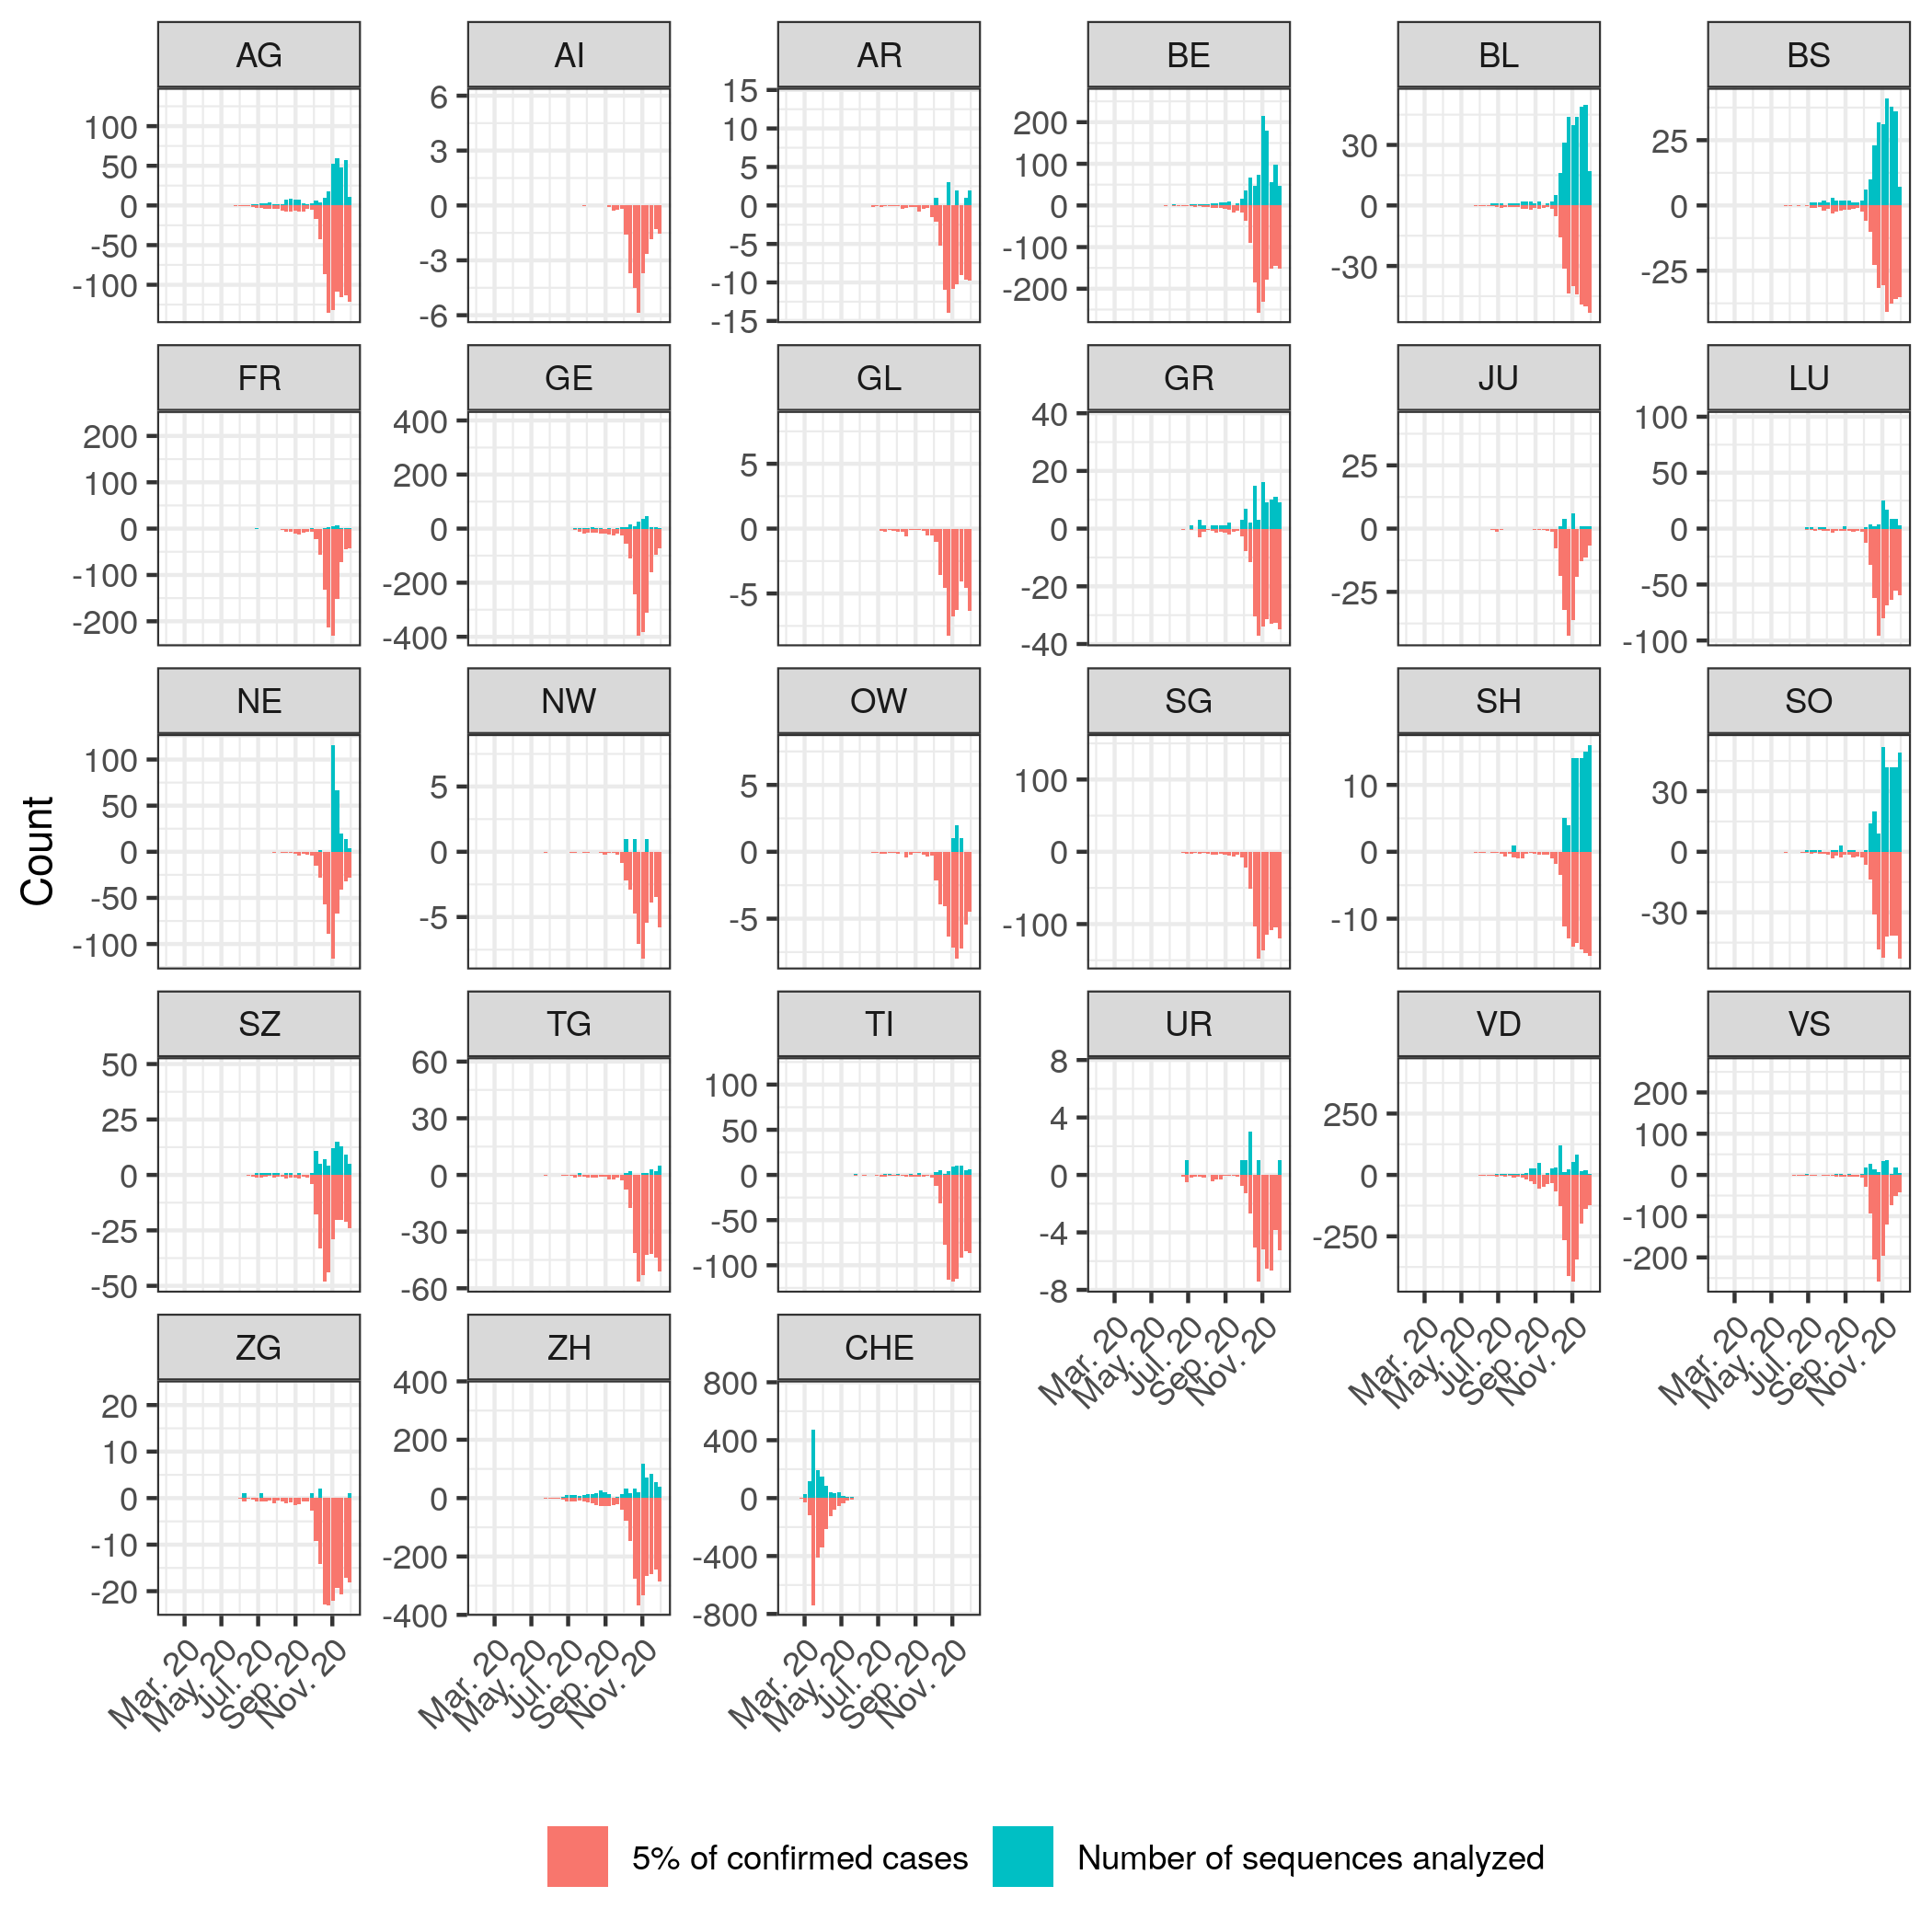
\includegraphics[width = 11.4cm]{figures/CHE_downsampling.png}
\caption{Spatio-temporal representativeness of analyzed genome sequences. The mirror y-axis aims to contrast temporal trends in confirmed cases (red) versus analyzed sequences (blue); all values are positive counts. Facet titles are standard abbreviations for Swiss cantons. 'CHE' represents Swiss-wide cases and sequences, since case count reporting by canton began mid-May 2020.}  
\label{fig:downsampling_representativeness}
\end{figure}

\begin{figure}
\centering
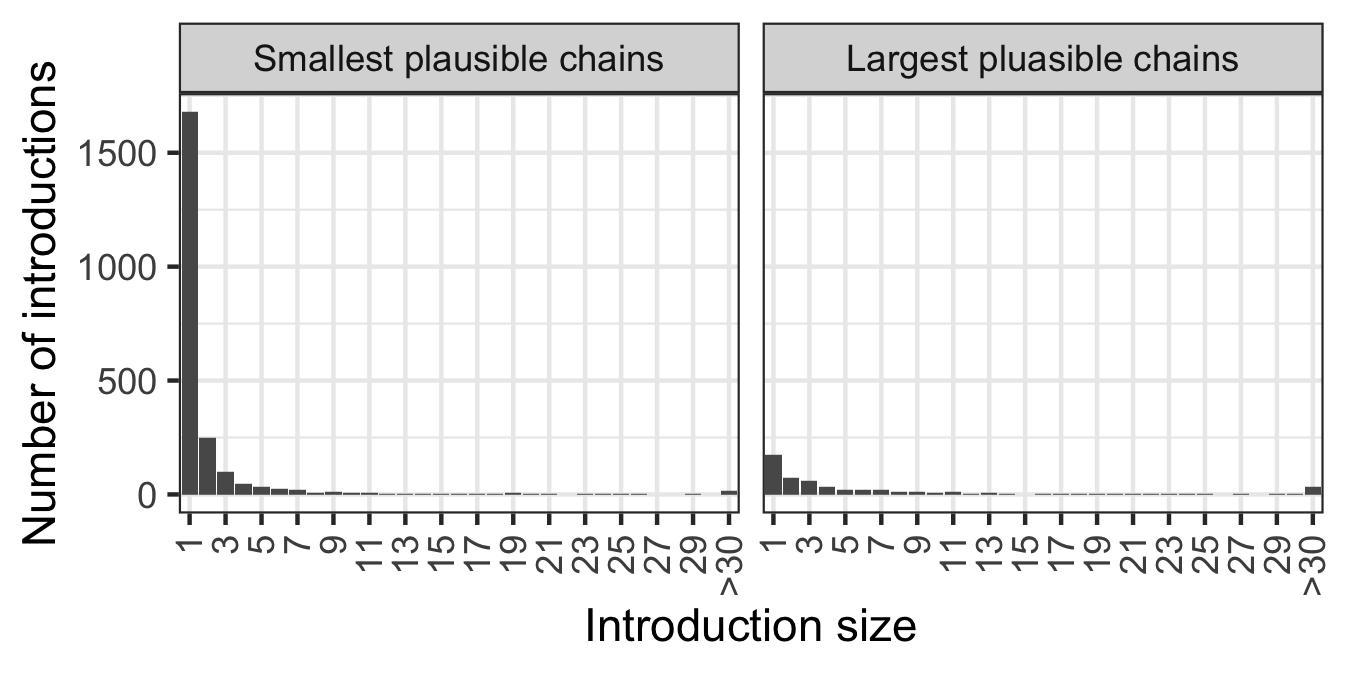
\includegraphics[width = 11.4cm]{figures/chain_size_dist.png}
\caption{Size distribution of estimated transmission chains.}  
\label{fig:chain_size_dist}
\end{figure}

\begin{figure}
\centering
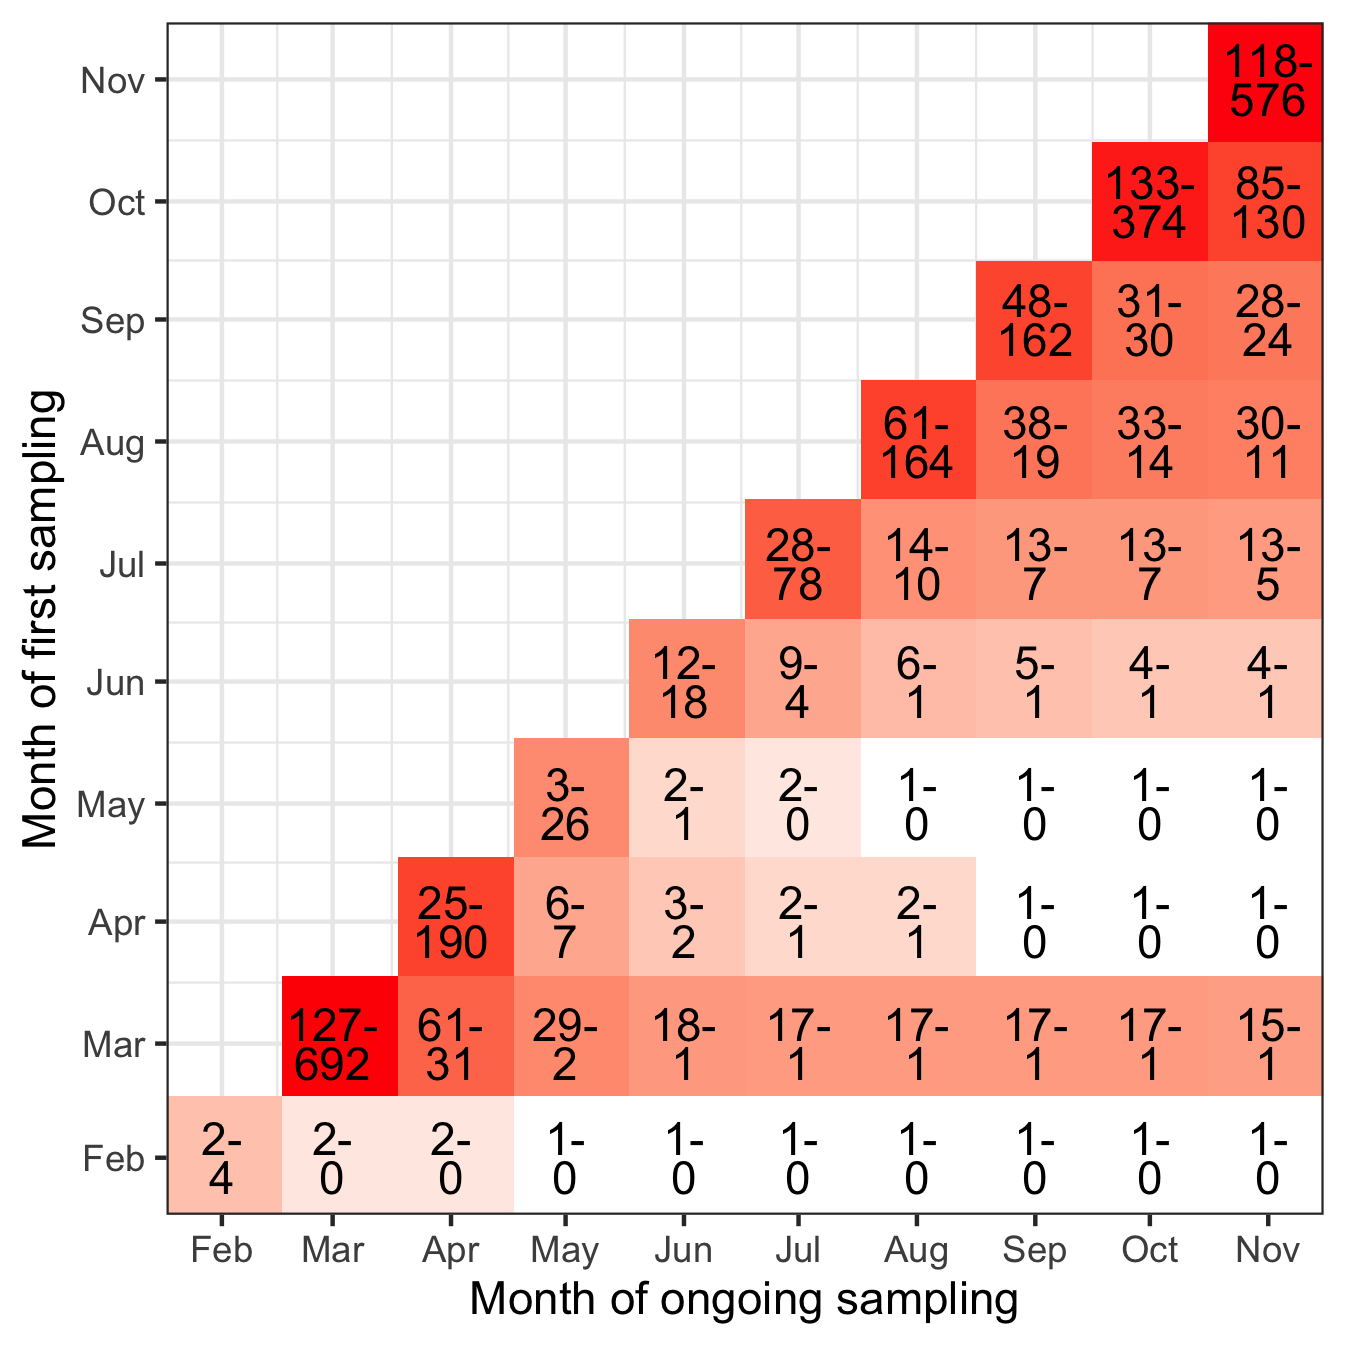
\includegraphics[width = 11.4cm]{figures/chain_longevity_matrix.png}
\caption{Heatmap of the number of newly sampled introductions each month (diagonal entries) and the number continuing to persisting into each following month (off-diagonal entries). Introduction are counted once in the month they are first sampled (``Month of first sampling'') and one every following month (``Month of ongoing sampling'') until the date of the latest sample. The ranges are between two point estimates generated assuming either few or many introductions.}  
\label{fig:chain-longevity-matrix}
\end{figure}

\begin{figure}
\centering
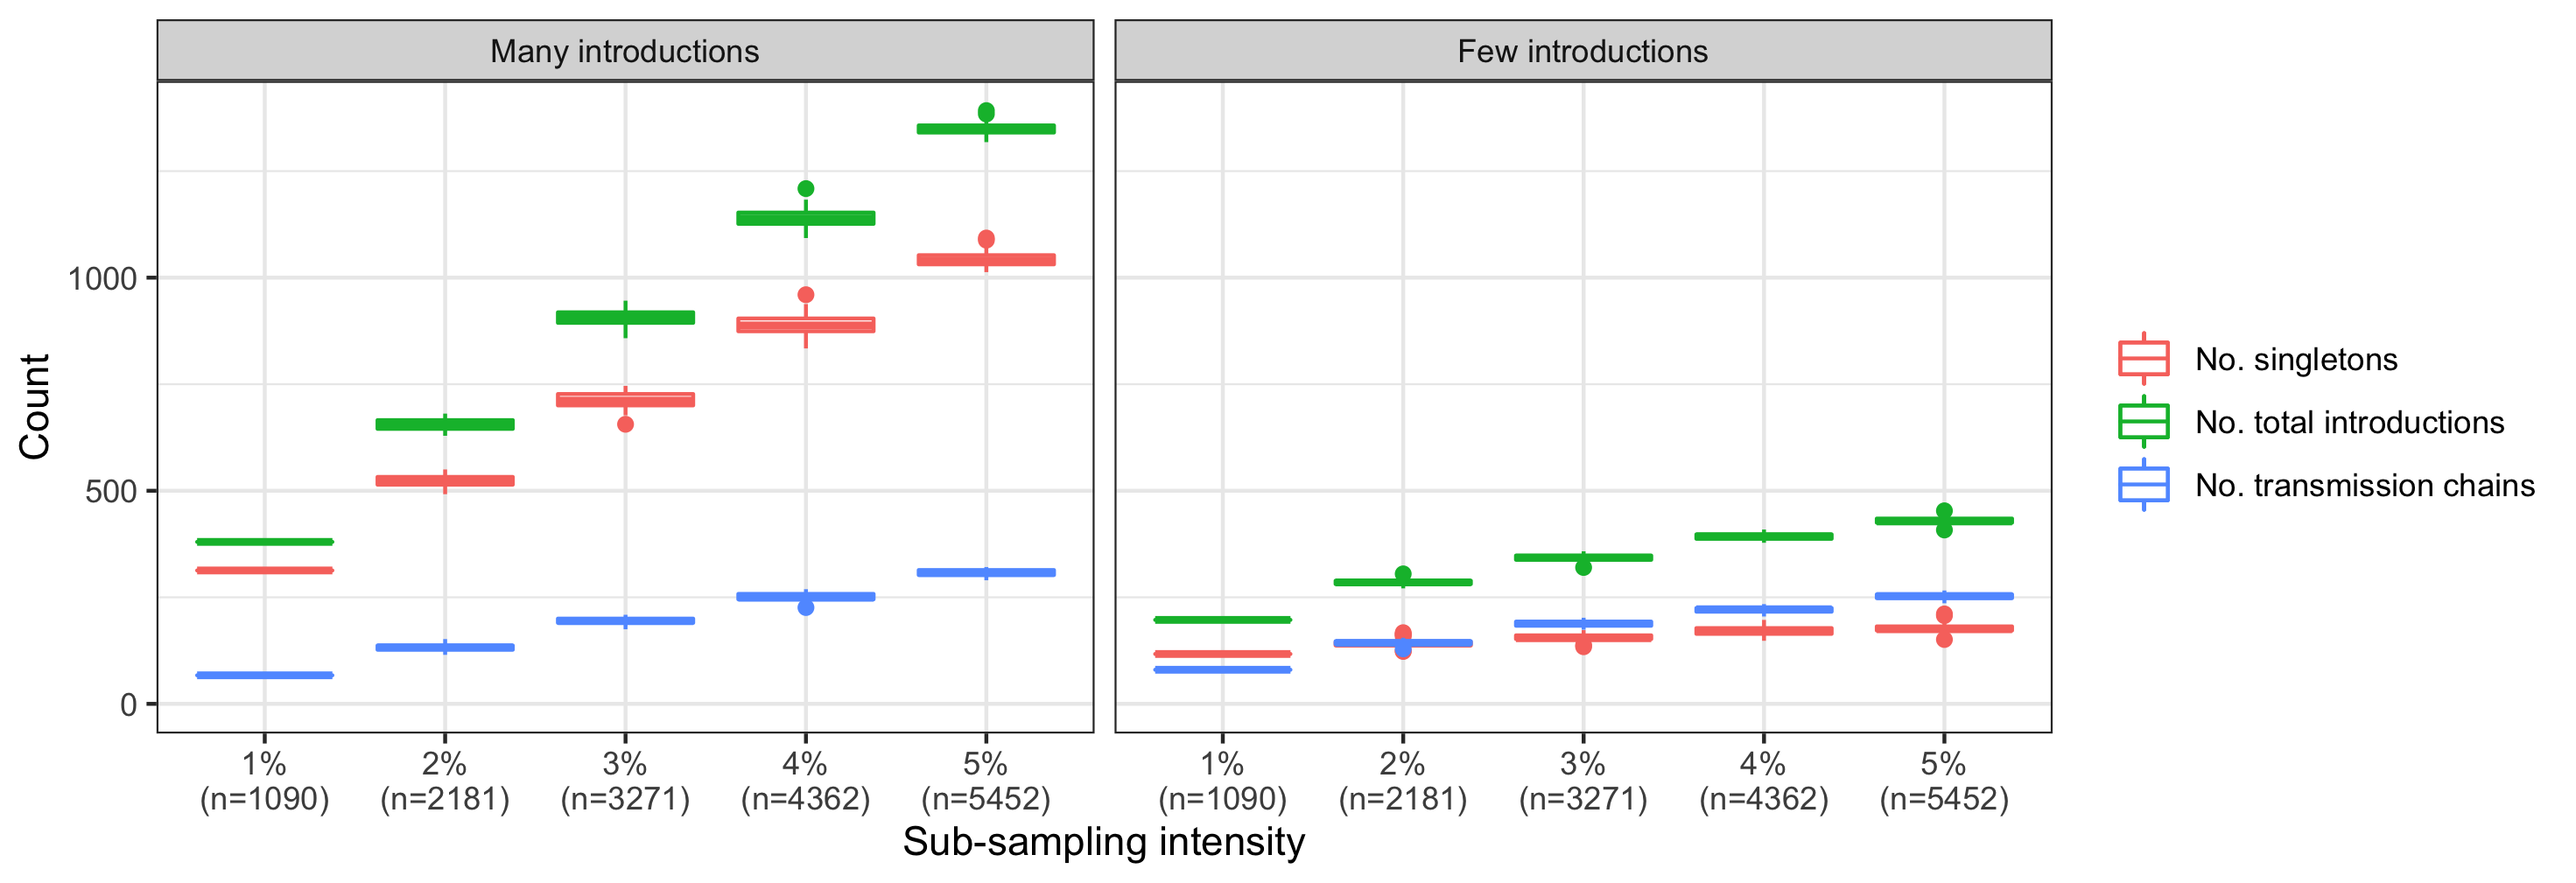
\includegraphics[width = 11.4cm]{figures/fig_SX_sensitivity_subsampling.png}
\caption{Number of estimated introductions as a function of the fraction of Swiss confirmed cases analyzed.}  
\label{fig:sensitivity_downsampling}
\end{figure}

\begin{figure}
\centering
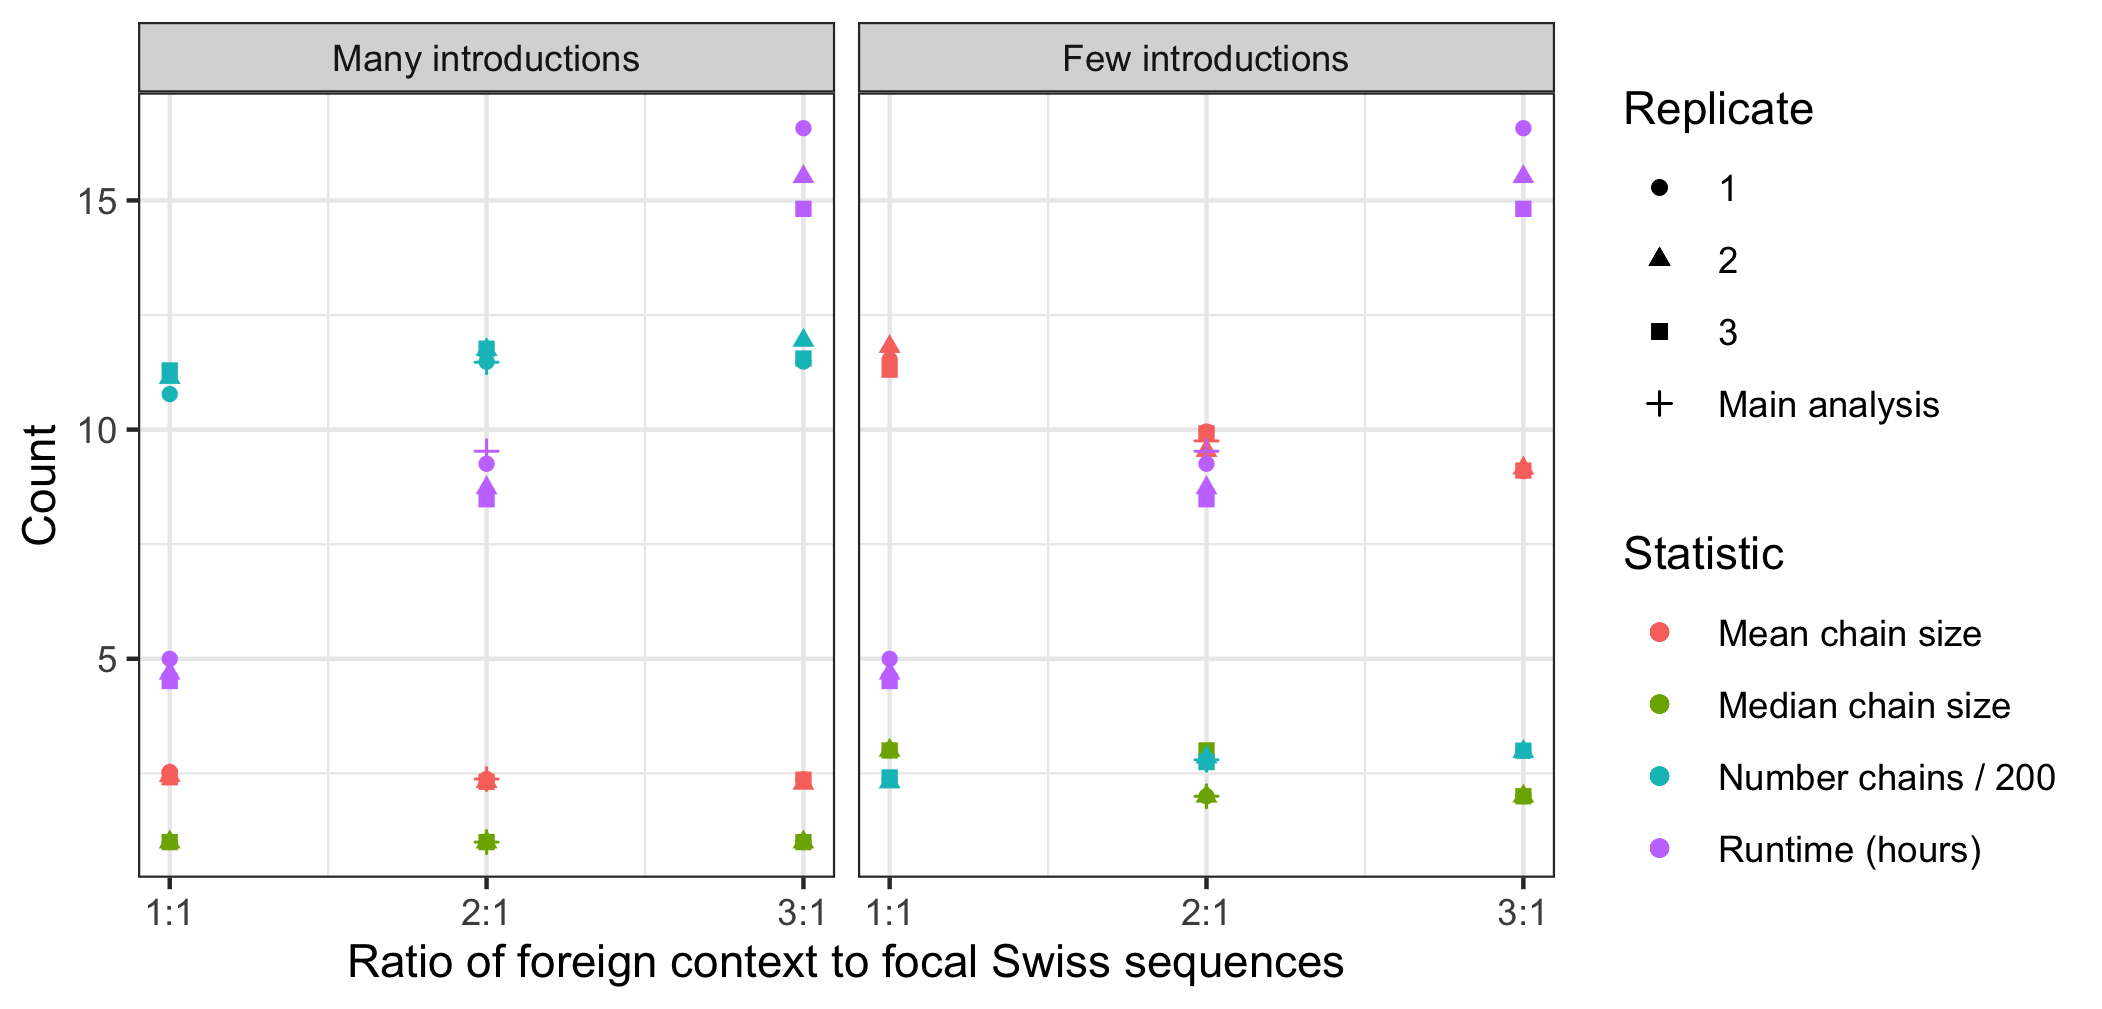
\includegraphics[width = 11.4cm]{figures/fig_SX_sensitivity_context_set_size.png}
\caption{Sensitivity of transmission chain summary statistics to different ratios of focal Swiss sequences to genetically similar foreign context sequences (1:1, 1:2, and 1:3).}  
\label{fig:sensitivity_context_set_size}
\end{figure}

\begin{figure}
\centering
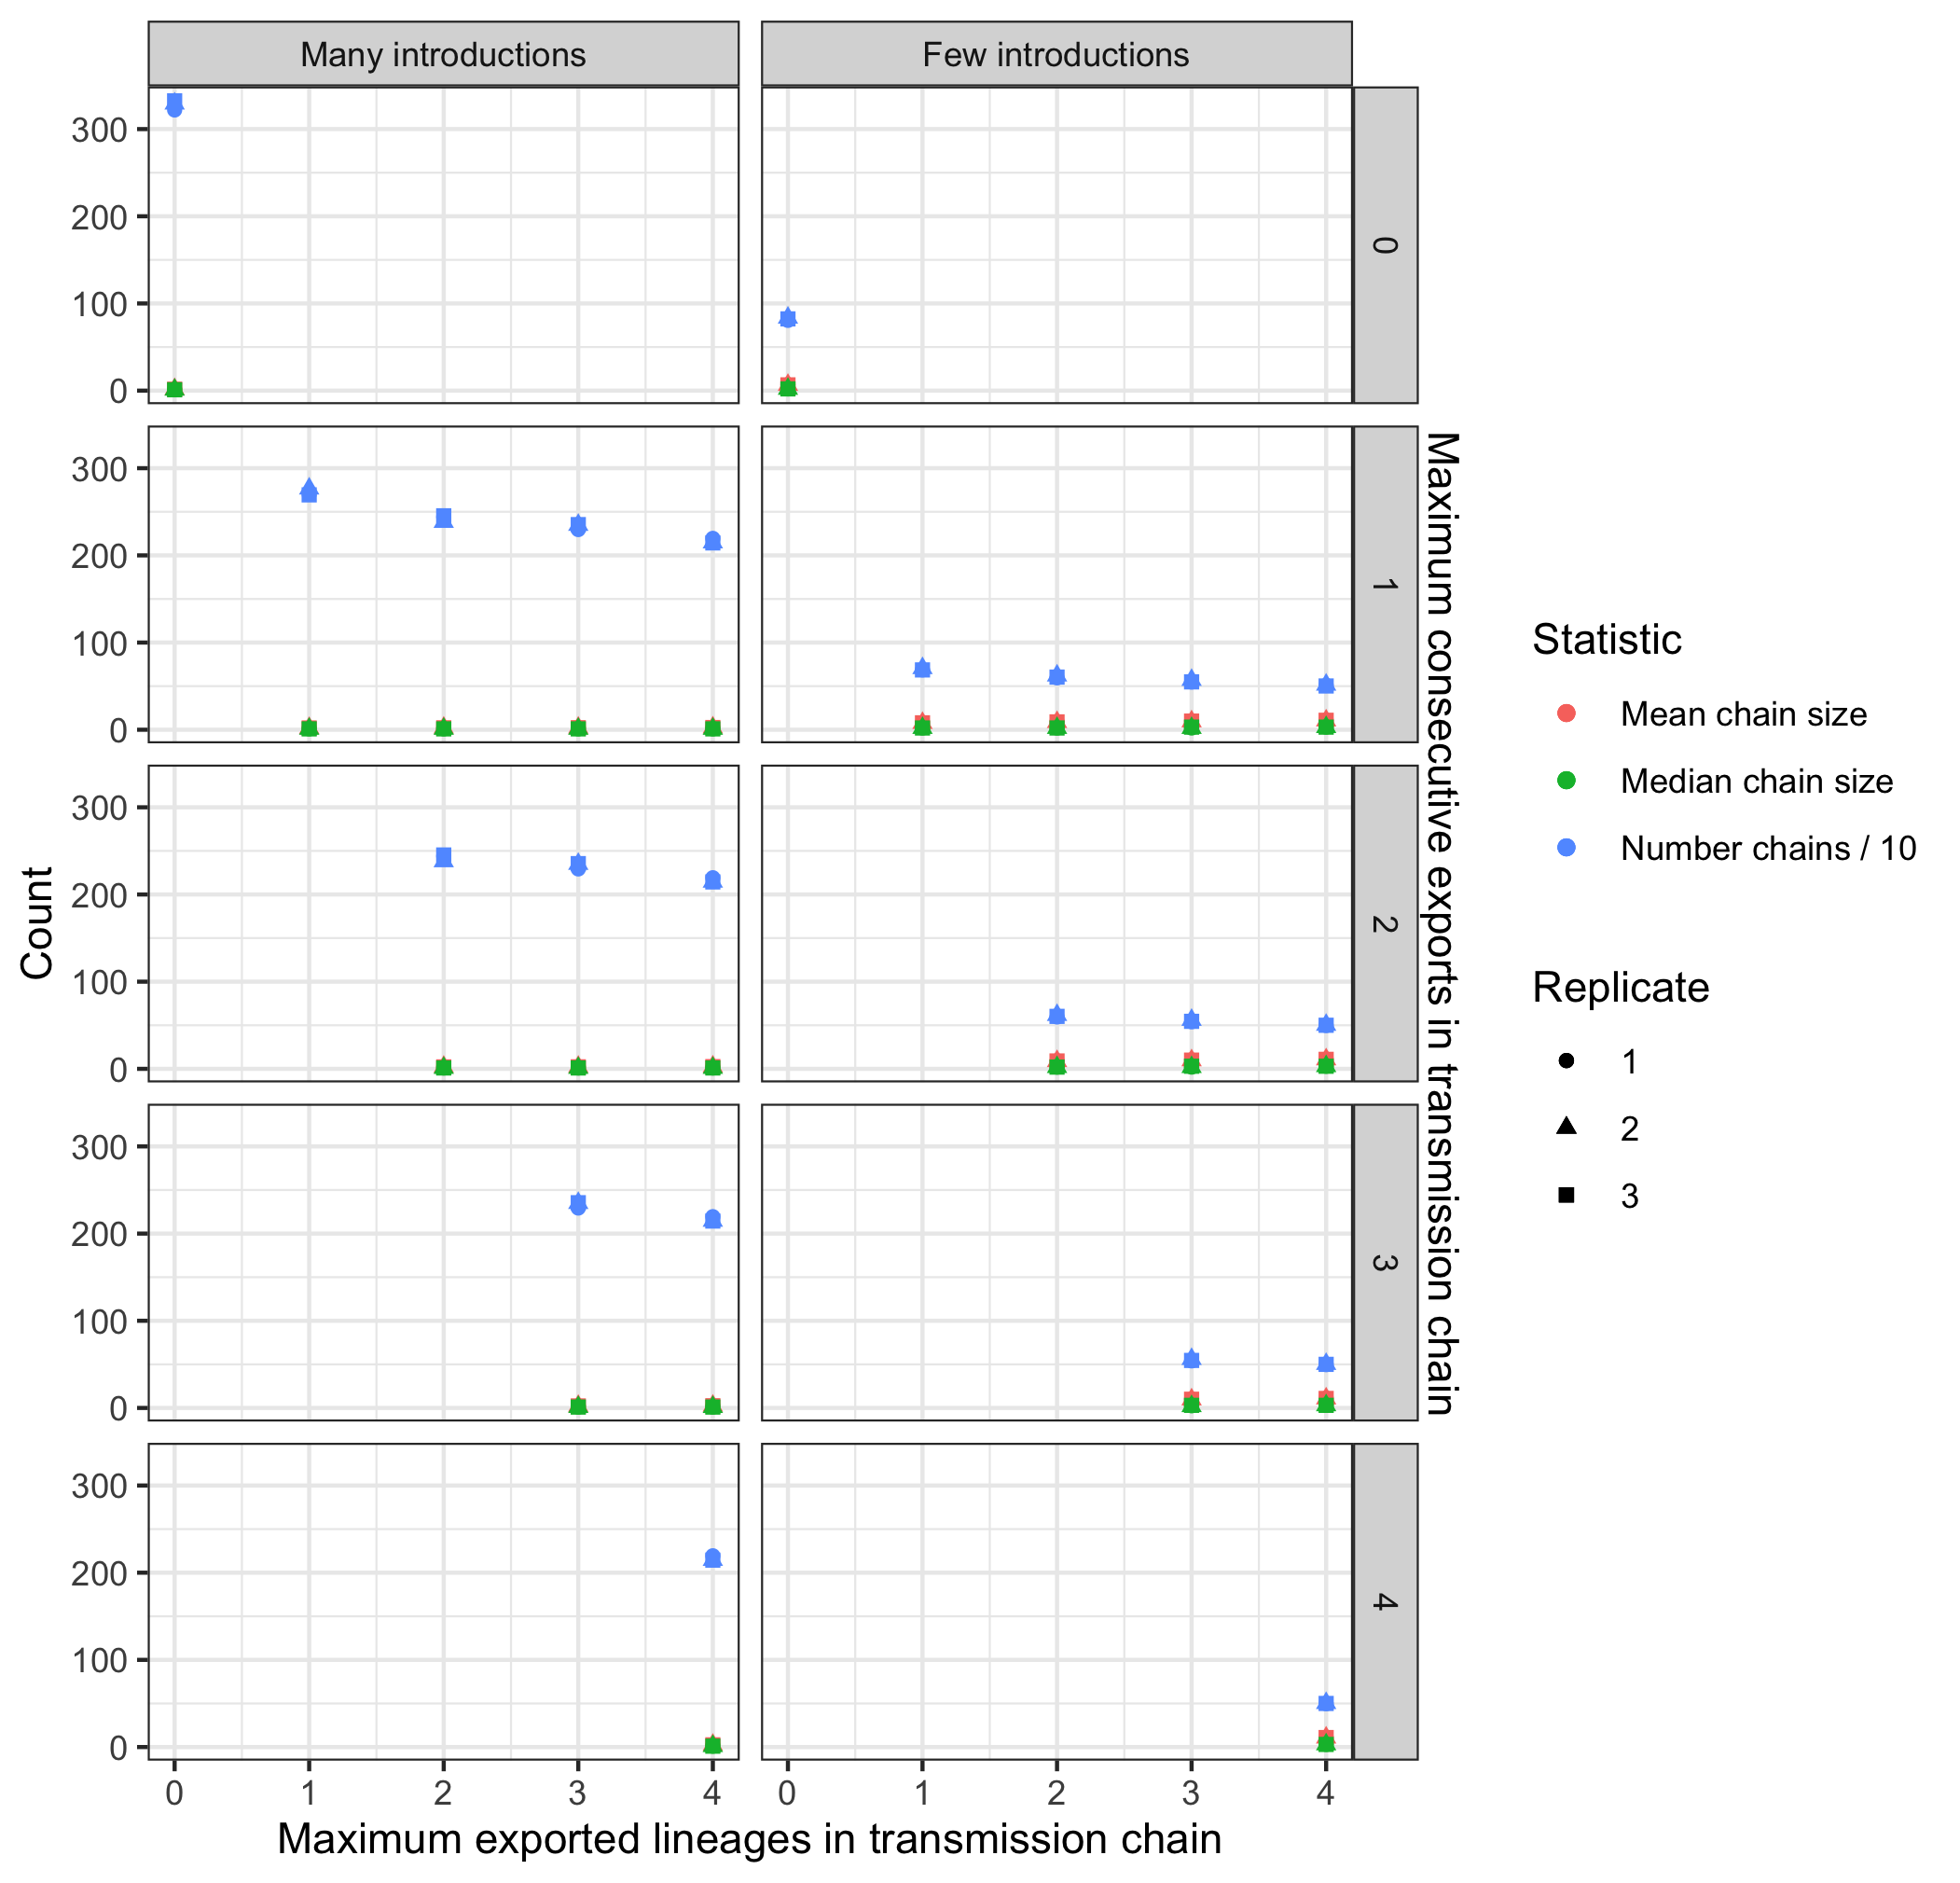
\includegraphics[width = 11.4cm]{figures/fig_SX_sensitivity_chain_defn.png}
\caption{Sensitivity of transmission chain summary statistics to different definitions of a transmission chain.}  
\label{fig:sensitivity_m_p}
\end{figure}

\begin{figure}[tbhp]
\centering
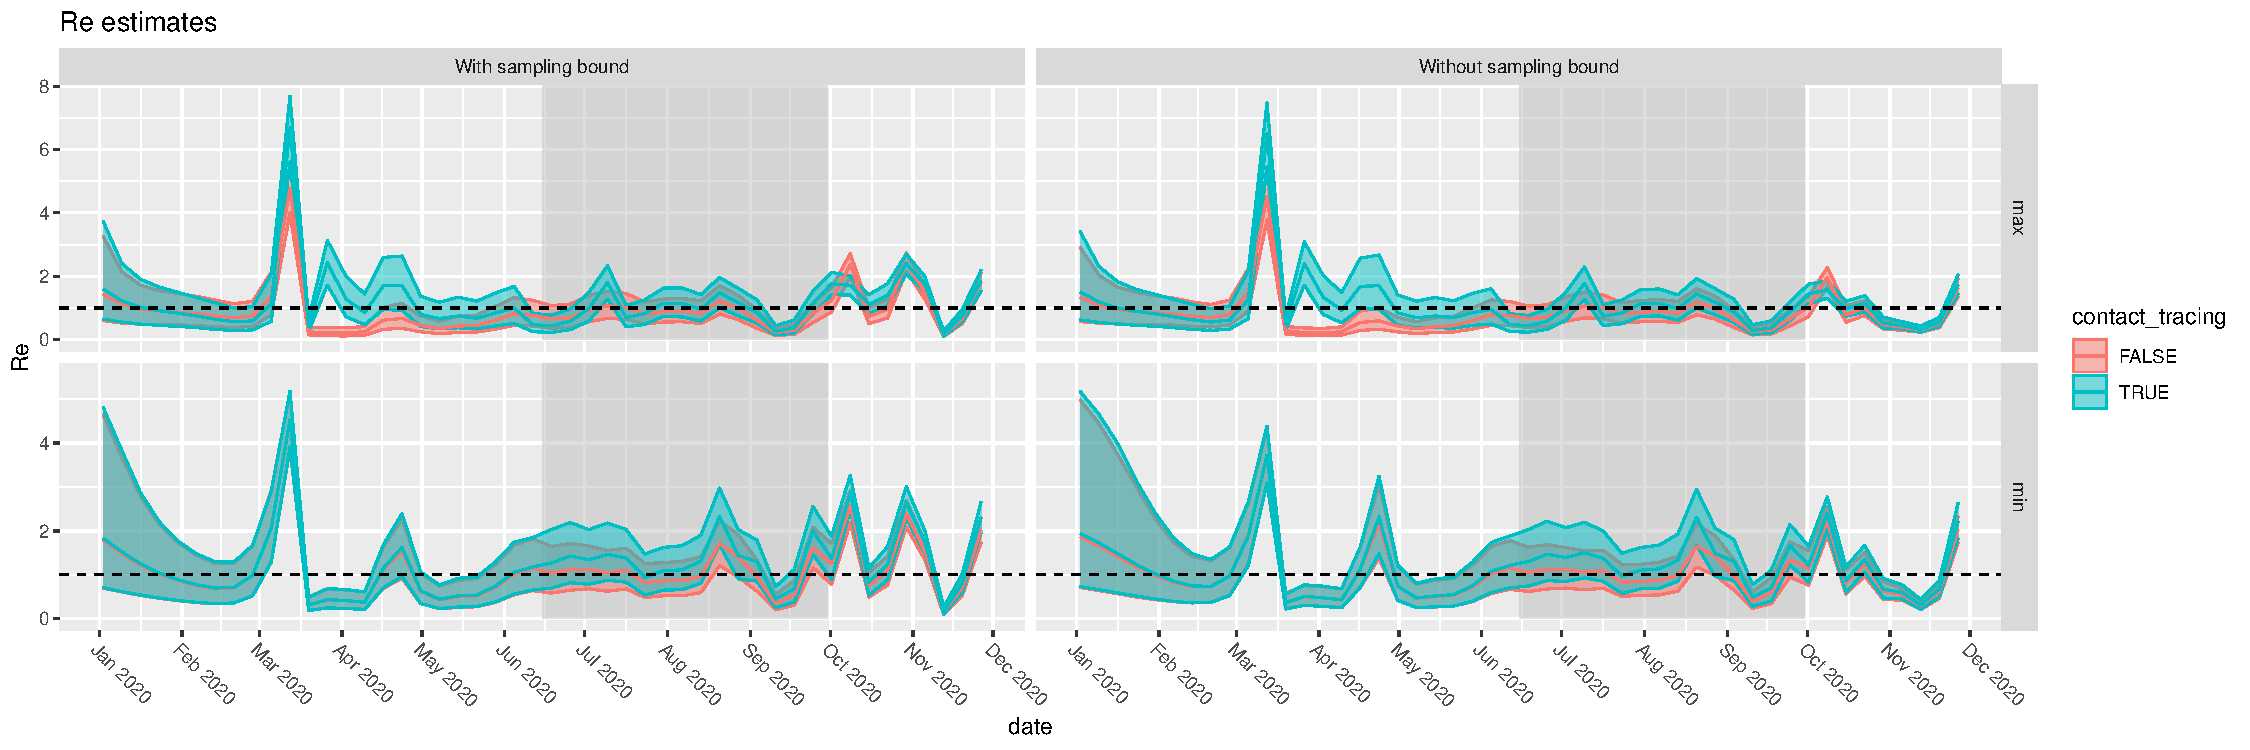
\includegraphics[width=\linewidth]{figures/bdsky_2021-08-18/Re_CHE_1deme.pdf}
\vfill
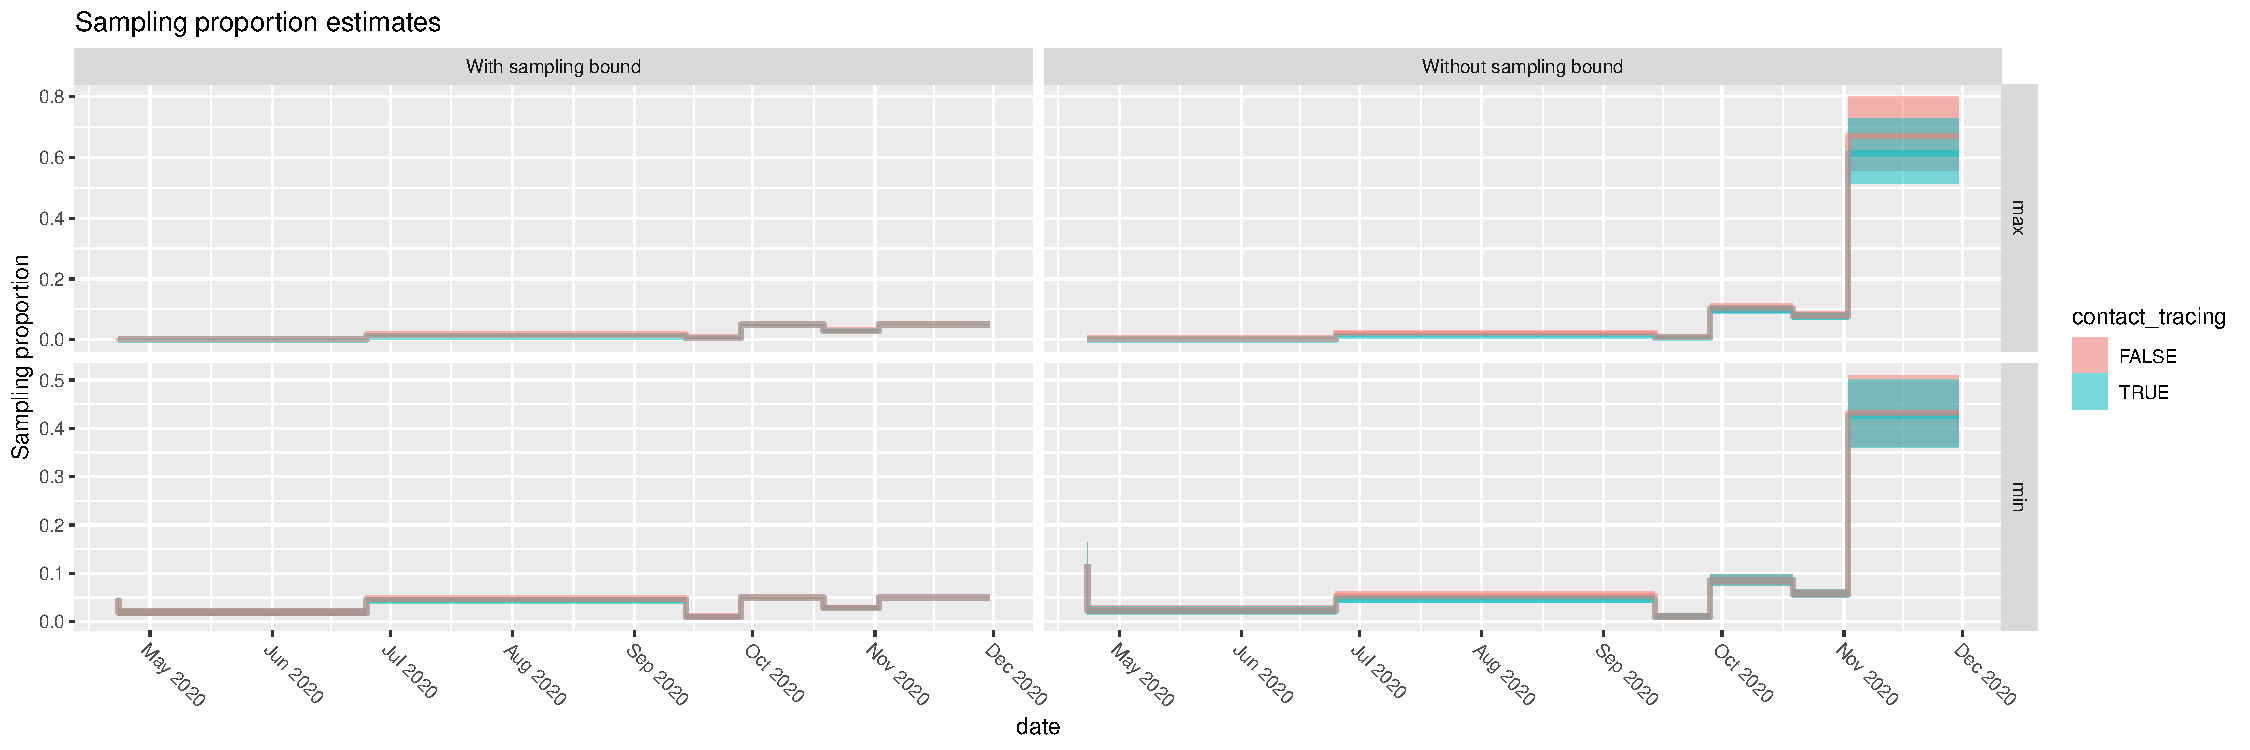
\includegraphics[width=\linewidth]{figures/bdsky_2021-08-18/sampProp_CHE_1deme.pdf}
\caption{Phylodynamic estimates for the time-varying effective reproductive number (top) and sampling proportion (bottom) in Switzerland under the base model with a damping factor, with and without bounded sampling.}  
\label{fig:1DemeCHResults}
\end{figure}
% Remember Re plot is now background Re (without contact tracing) and no longer the actual average Re

\begin{figure}[tbhp]
\centering
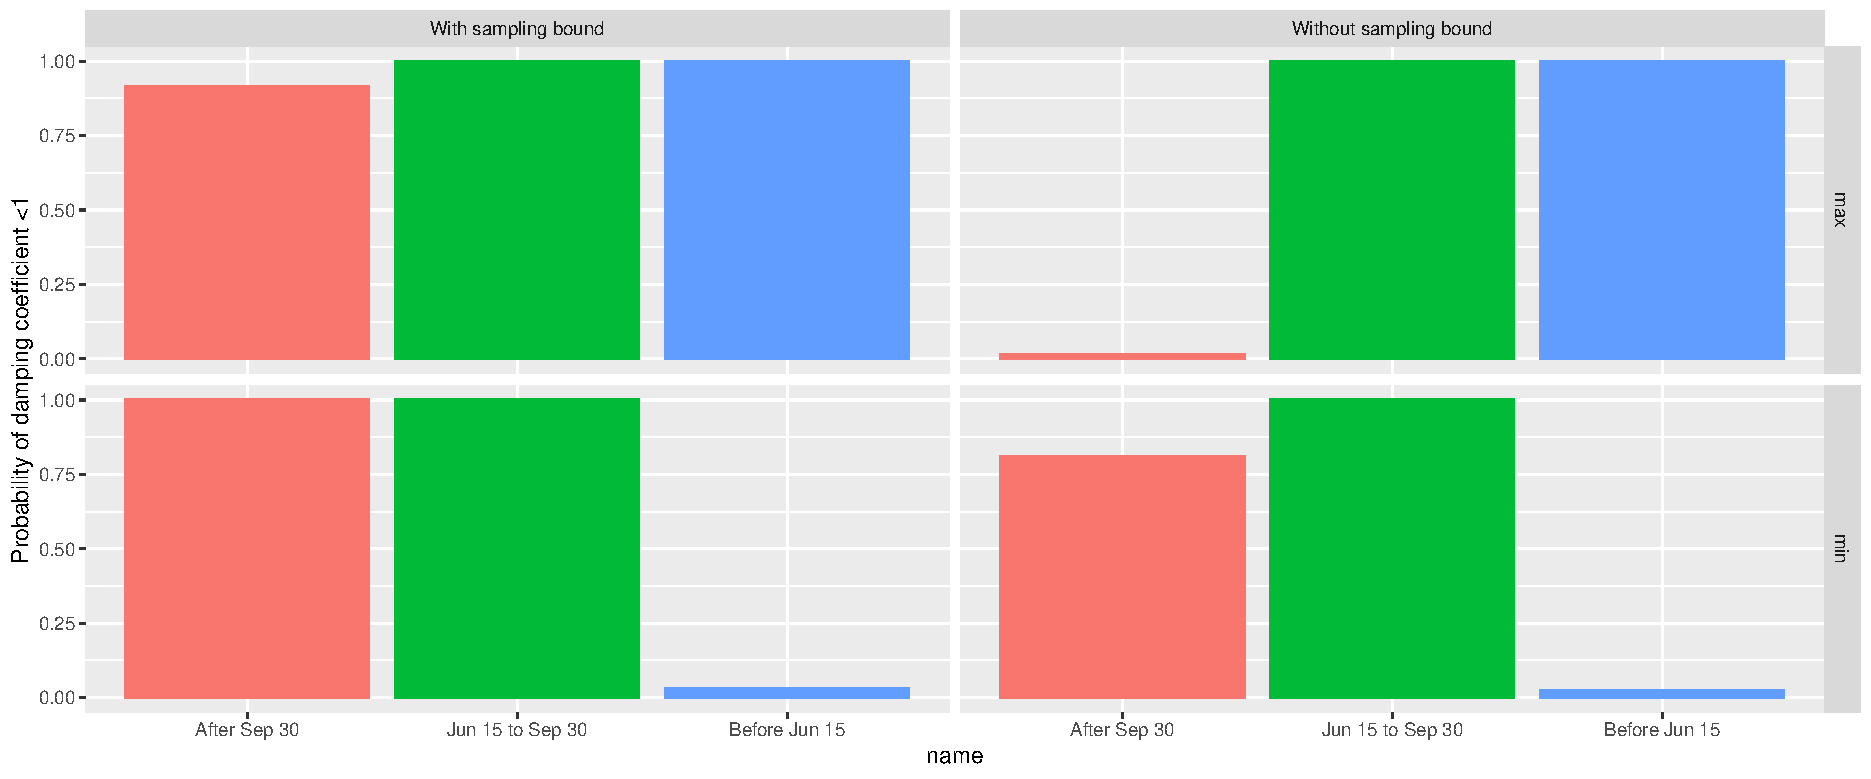
\includegraphics[width=0.4\linewidth]{figures/bdsky_2021-08-18/CT_dampingProbs_CHE_1deme.pdf}
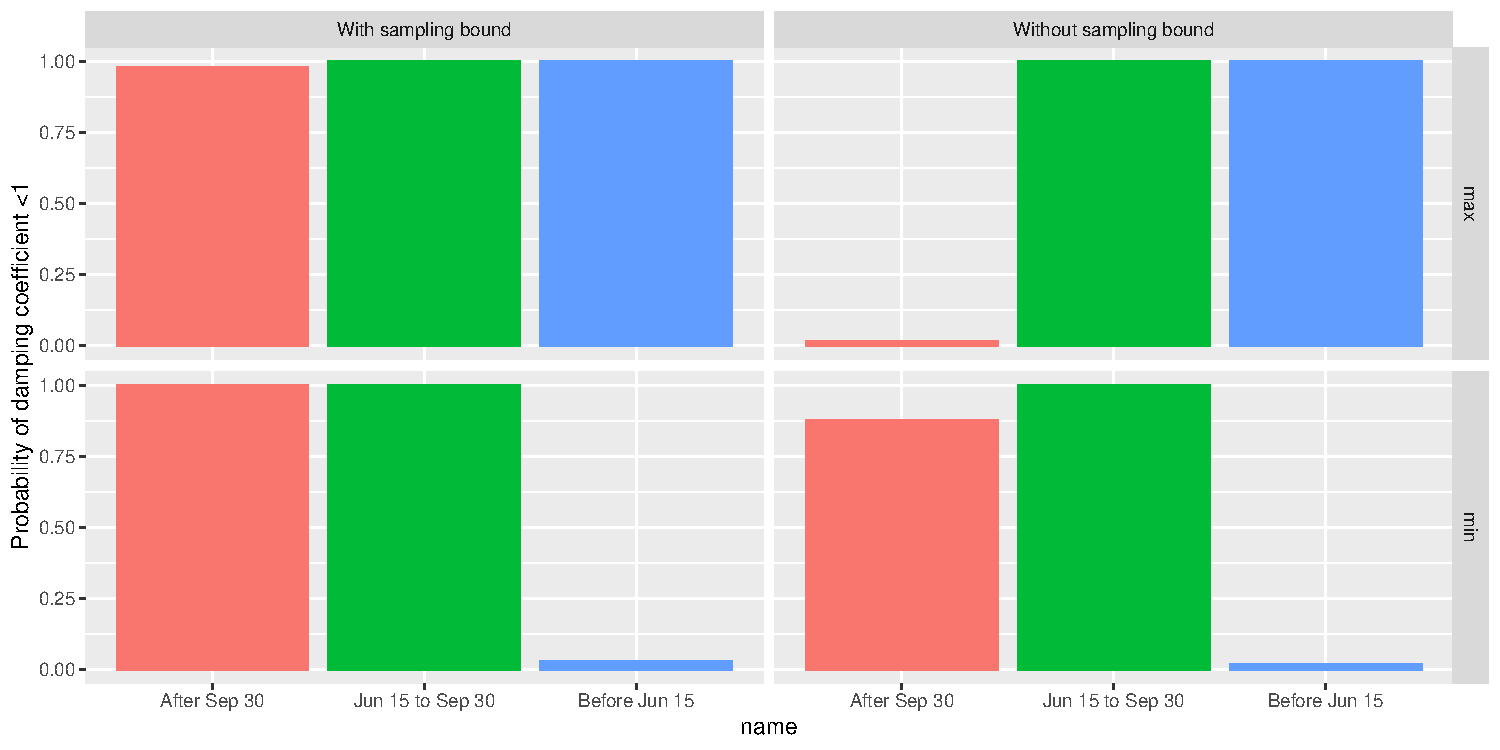
\includegraphics[width=0.4\linewidth]{figures/bdsky_2021-08-18/CT_dampingProbs_2deme.pdf}
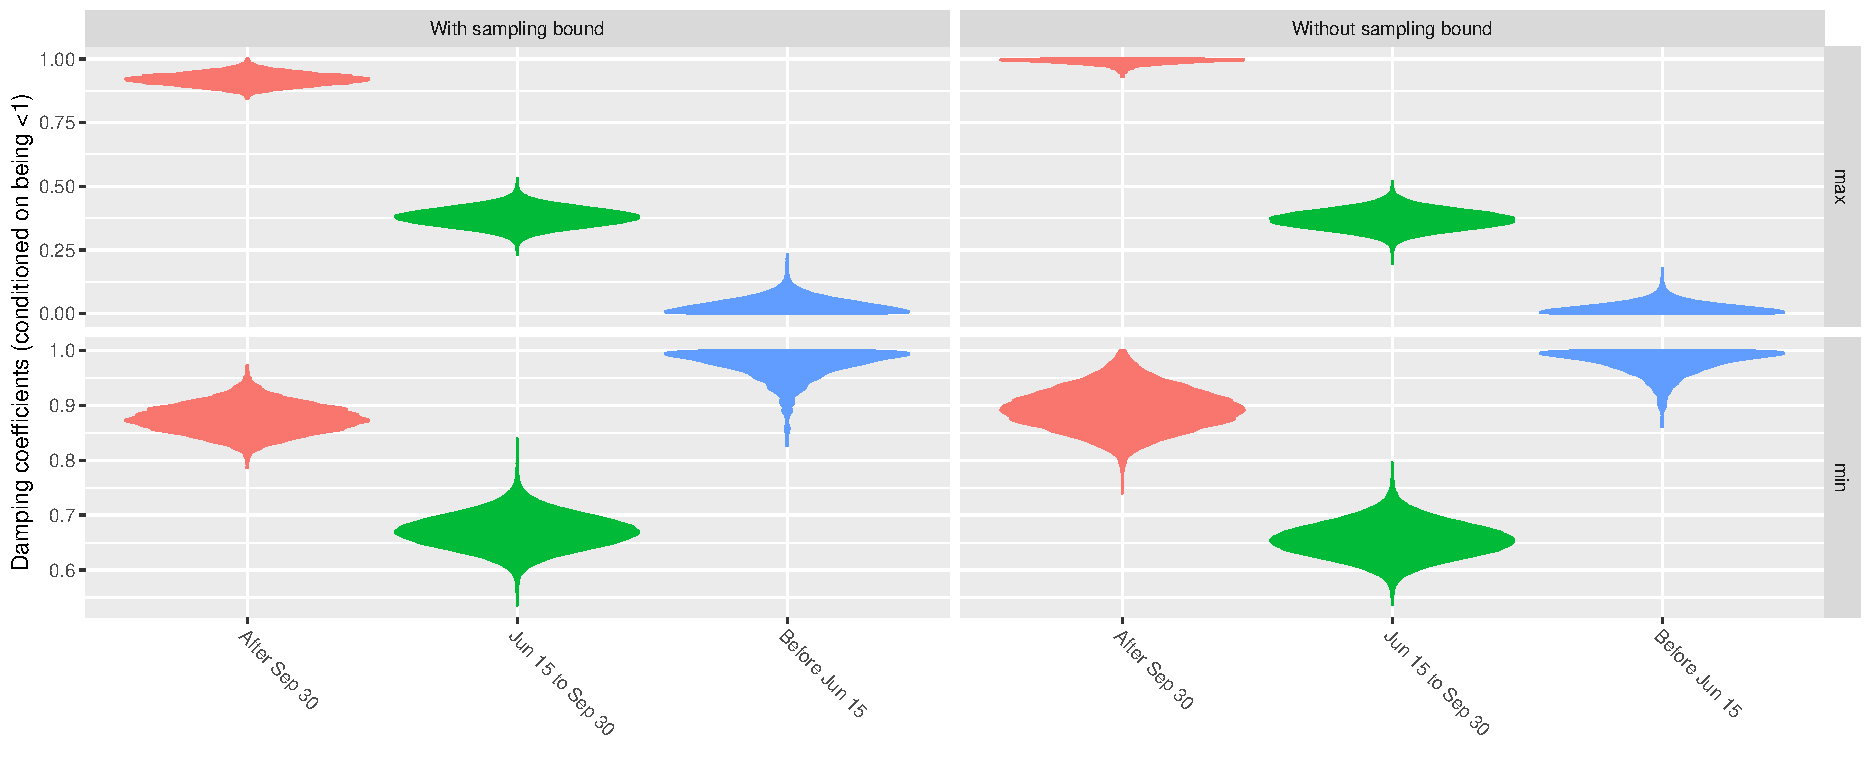
\includegraphics[width=0.4\linewidth]{figures/bdsky_2021-08-18/CT_conditionedDamping_CHE_1deme.pdf}
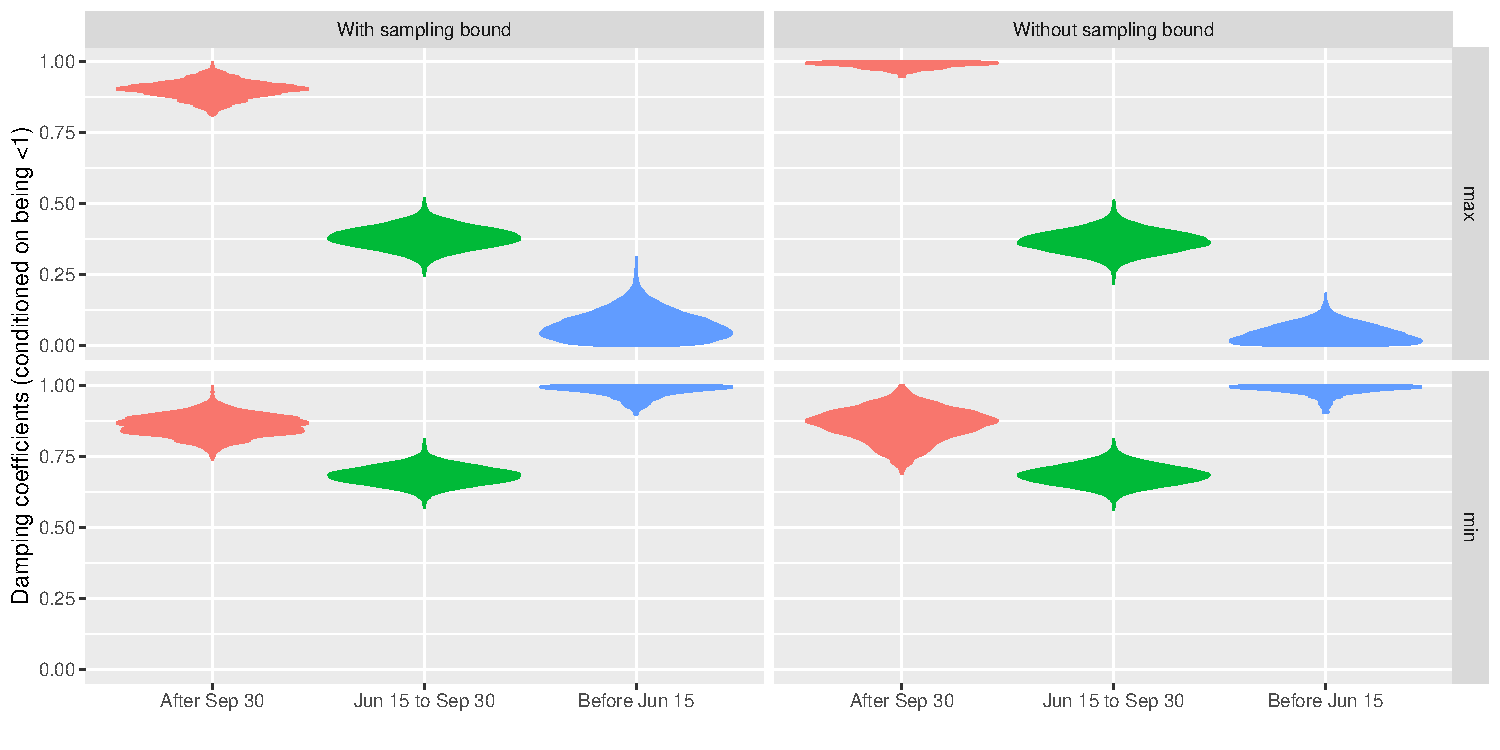
\includegraphics[width=0.4\linewidth]{figures/bdsky_2021-08-18/CT_conditionedDamping_2deme.pdf}
\caption{Phylodynamic estimates for the damping factor in Switzerland. Top is inclusion probability for the damping factor, bottom is dampling factor estimate conditioned on inclusion. Left are inferences under the base model and right are inferences under the base model with a SS (super-spreading) deme.}  
\label{fig:1vs2demeDampingFactorResults}
\end{figure}
\newpage

\begin{figure}[tbhp]
\centering
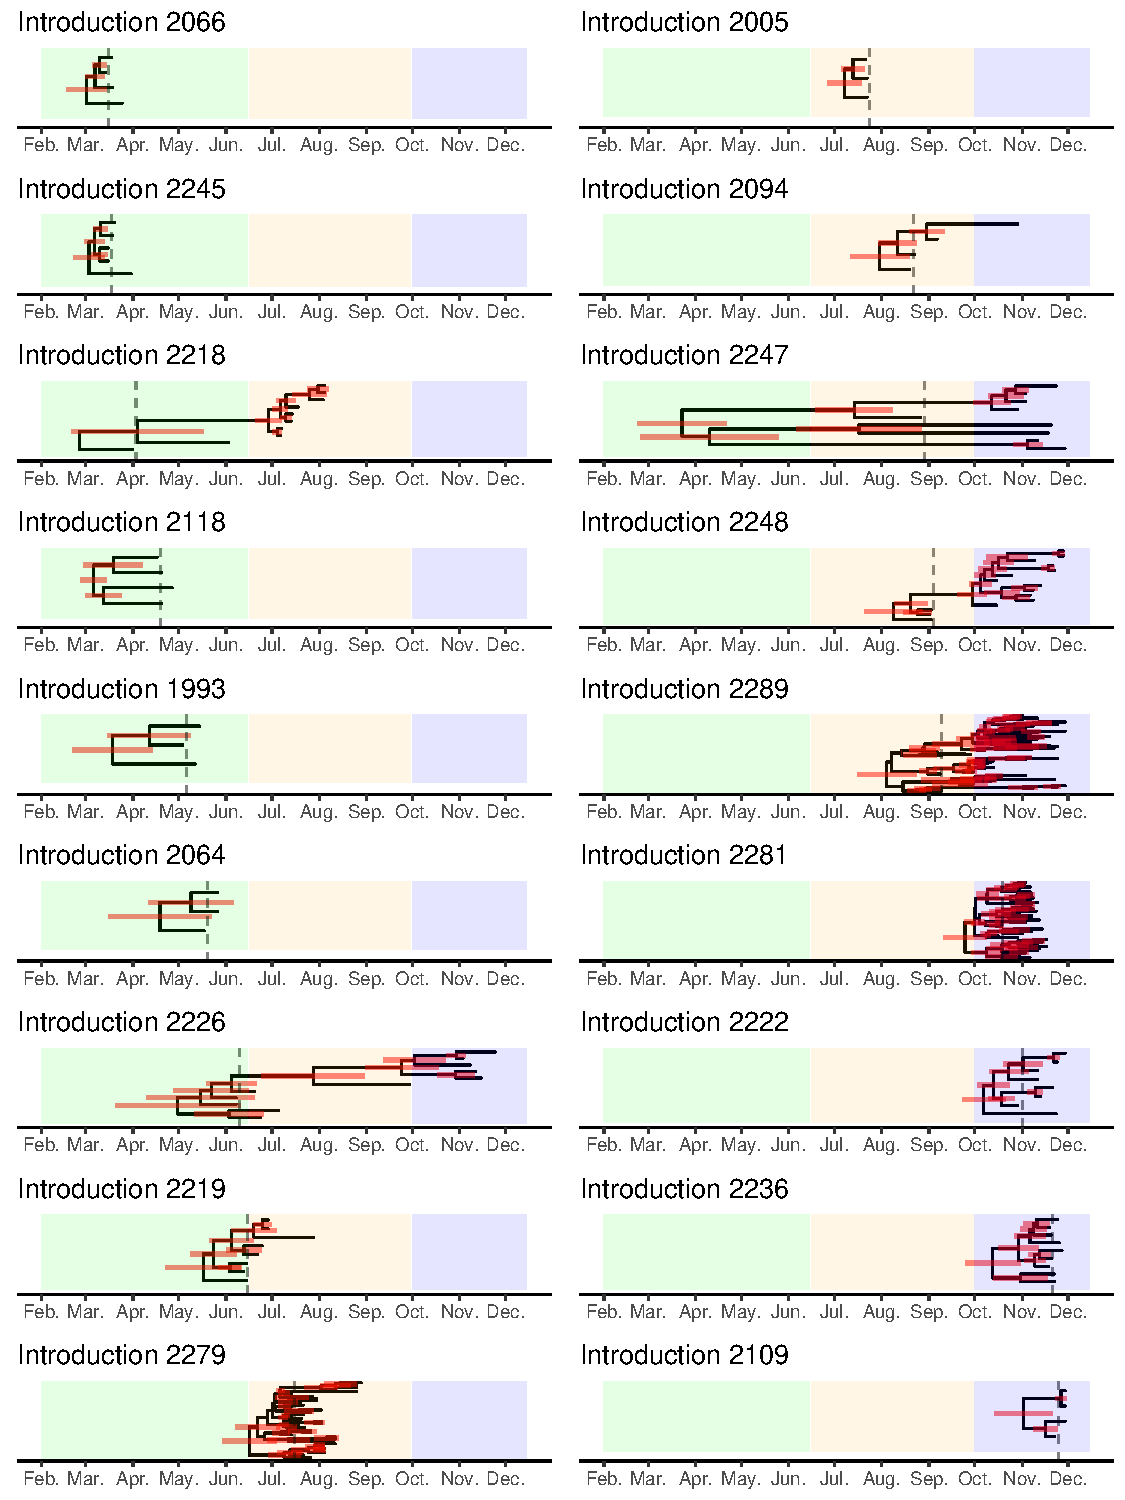
\includegraphics[width=0.75\linewidth]{figures/bdsky_2021-08-18/Re_skyline.max_chains.sampUB1.0.ctEst1.summary_trees.pdf}
\caption{Summary trees from the phylodynamic analysis for Switzerland. Here introductions were estimated assuming ``many'' introductions. The 50th and 95th percentile largest introductions among those first sampled each month are shown. The three color regions represent the Spring (green), Summer (orange) and Fall (blue) periods. The vertical dashed line shows the date at which the transmission rate can slow for each introduction - two days after the first sample date. The red bars show the 95\% highest posterior density uncertainty in node dates.}  
\label{fig:logged-chains}
\end{figure}
\newpage

\begin{figure}[tbhp]
\centering
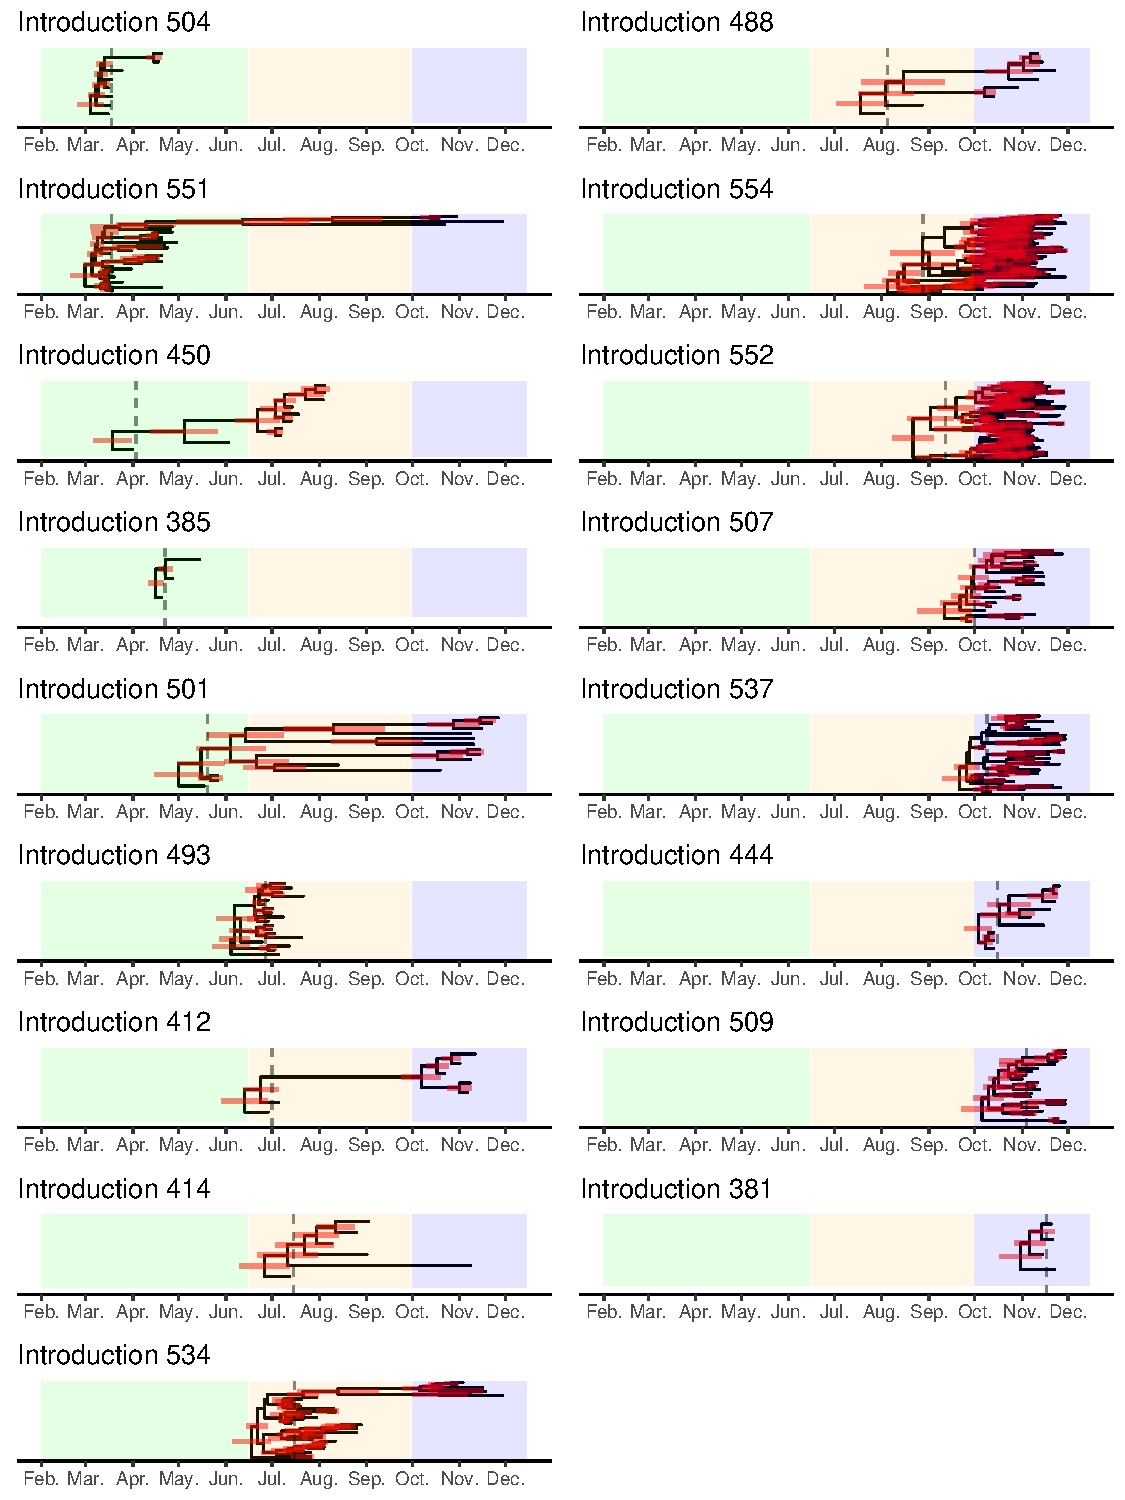
\includegraphics[width=0.75\linewidth]{figures/bdsky_2021-08-18/Re_skyline.min_chains.sampUB1.0.ctEst1.summary_trees.pdf}
\caption{Summary trees from the phylodynamic analysis for Switzerland. Here introductions were estimated assuming ``few'' introductions. The 50th and 95th percentile largest introductions among those first sampled each month are shown. The three color regions represent the Spring (green), Summer (orange) and Fall (blue) periods. The vertical dashed line shows the date at which the transmission rate can slow for each introduction - two days after the first sample date. The red bars show the 95\% highest posterior density uncertainty in node dates.}  
\label{fig:logged-chains}
\end{figure}
\newpage

\begin{figure}[tbhp]
\centering
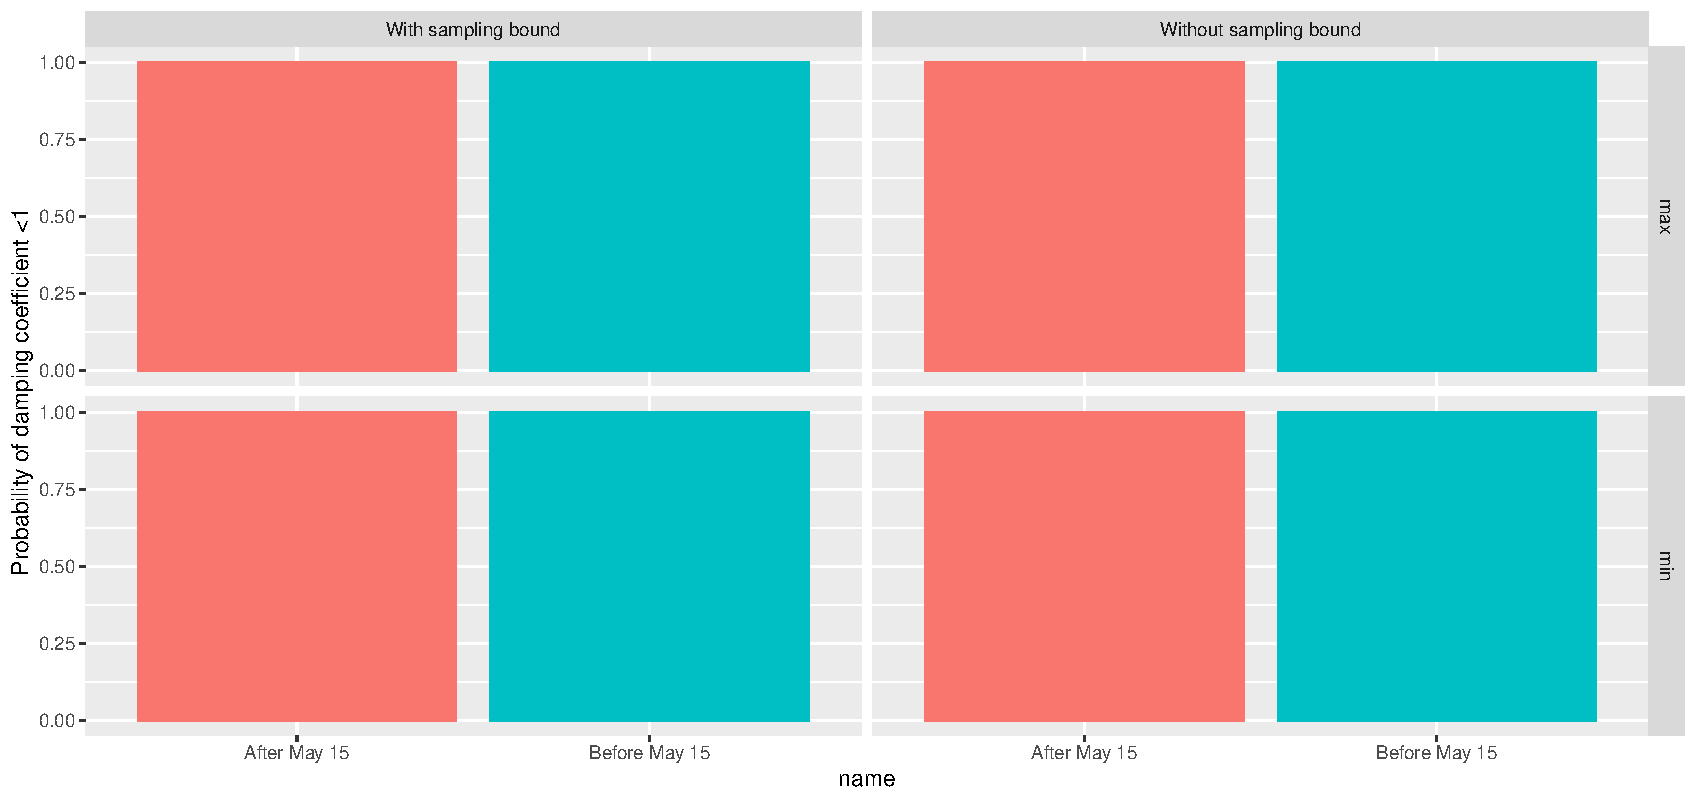
\includegraphics[width=\linewidth]{figures/bdsky_2021-08-18/CT_dampingProbs_NZL.pdf}
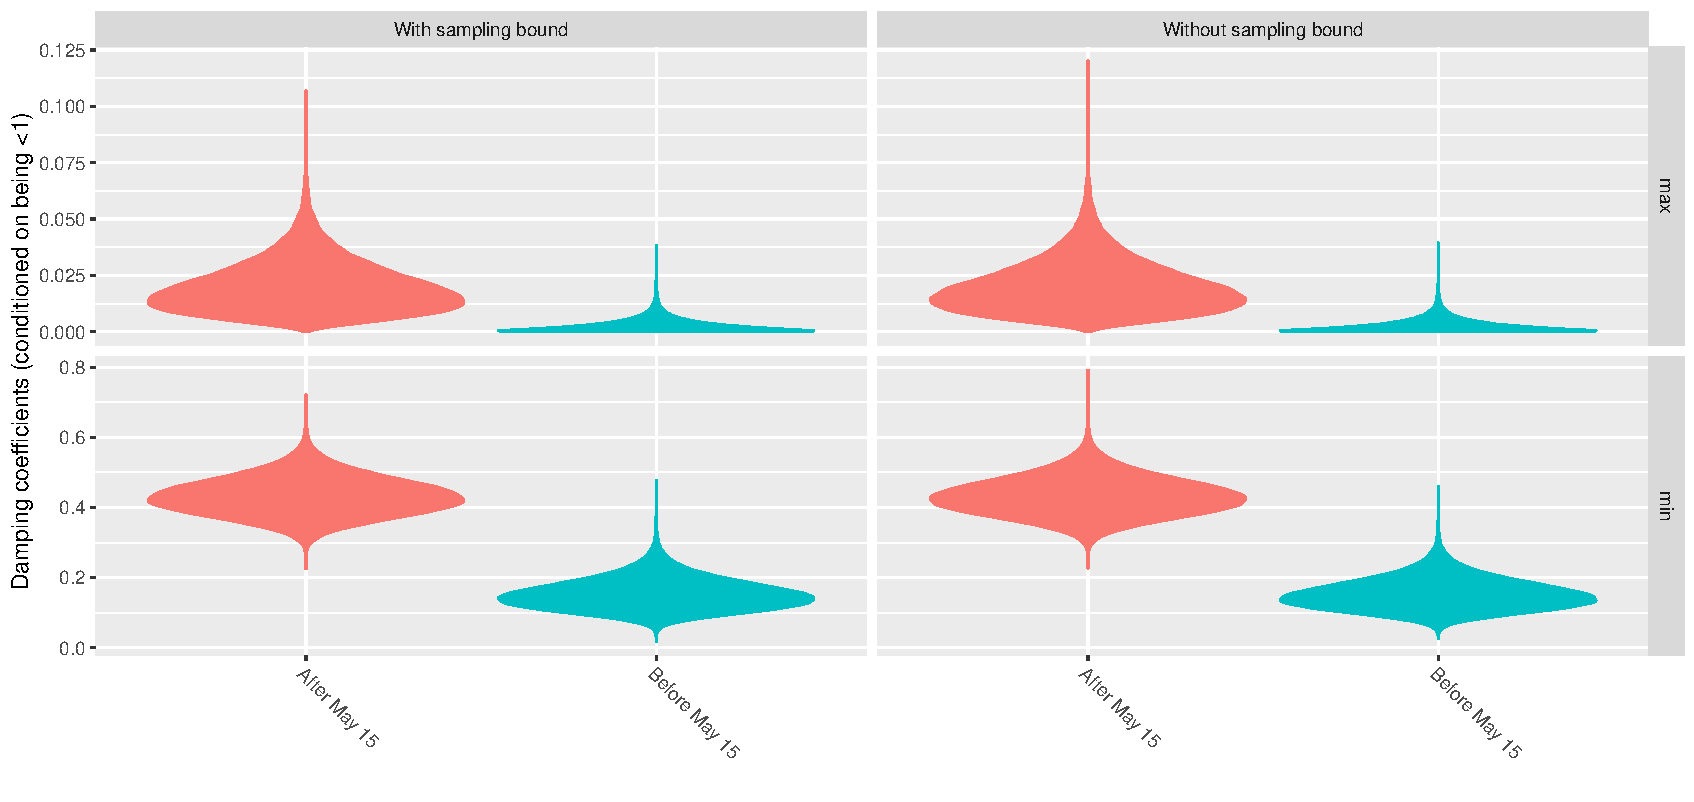
\includegraphics[width=\linewidth]{figures/bdsky_2021-08-18/CT_conditionedDamping_NZL.pdf}
\caption{Phylodynamic estimates for the damping factor in New Zealand. Top is inclusion probability for the damping factor, bottom is dampling factor estimate conditioned on inclusion.}  
\label{fig:NZLDampingFactorResults}
\end{figure}
\newpage

\begin{table}[H]
\caption{Various phylodynamic models employed for the main analysis and sensitivity checks.}
\label{tab:phylo-models}
\begin{tabular}{cccccc}
Data set & Polytomy resolution & Damping factor (contact\_tracing) & Damping factor + SS Deme & Damping factor + Sampling bound \\
\midrule
Swiss & Many introductions (max) & Y & Y & Y \\
Swiss & Few introductions (min) & Y & Y & Y \\
New Zealand & Many introductions (max) & Y & & \\
New Zealand & Few introductions (min) & Y & & \\
\bottomrule
\end{tabular}
\newline
\addtabletext{Models with a ``Damping factor'' include a parameter representing a possible transmission slow-down upon sampling. Models with a ``SS deme'' include a second deme representing super-spreaders. Models with ``Sampling bound'' have the sampling proportion restricted to be less than the number of genomes divided by the number of confirmed cases.}
\end{table}

\newpage
\begin{table}[H]
\centering
\caption{Sampling proportion change-points in the phylodynamic analyses.}
\begin{tabular}{lp{6cm}rr}
Start date & Description \\
\midrule
23. Apr 2020 & All symptomatic individuals can get tested \\
25. Jun 2020 & Government pays for tests for symptomatic individuals \\
14. Sept 2020 & Genome sampling $<<$ 5\% of confirmed cases \\
28. Sept 2020 & Number of tests conducted and \% positivity dramatically increase, genome sampling also increases \\
19. Oct 2020 & Genome sampling $<<$ 5\% of confirmed cases again \\
11. Nov 2020 & Genome sampling improves again \\
\bottomrule
\end{tabular}
\end{table}

\newpage
\begin{table}[H]
\caption{Contingency table for singleton introductions and transmission chains by time period assuming many (right) and few (left)  introductions.}
% latex table generated in R 4.0.5 by xtable 1.8-4 package
% Fri Jul 16 15:33:02 2021
\begin{tabular}{lcccc}
  \hline
 &  & Singleton & Transmission chain & Total \\ 
  \hline
1 & MRCA during lockdown & 470 &  73 & 543 \\ 
  2 & MRCA not during lockdown & 1208 & 497 & 1705 \\ 
  3 & Total & 1678 & 570 & 2248 \\ 
   \hline
\end{tabular}

% latex table generated in R 4.0.5 by xtable 1.8-4 package
% Fri Sep  3 16:31:51 2021
\begin{tabular}{lcccc}
  \hline
 &  & Singleton & Transmission chain & Total \\ 
  \hline
1 & MRCA during lockdown &  47 &  28 &  75 \\ 
  2 & MRCA not during lockdown & 152 & 332 & 484 \\ 
  3 & Total & 199 & 360 & 559 \\ 
   \hline
\end{tabular}

\label{tab:lockdown-contingency}
\end{table}

\newpage
% latex table generated in R 4.0.5 by xtable 1.8-4 package
% Tue Jul  6 13:30:28 2021
\begin{longtable}{lp{4cm}ccc}
  \hline
 & Lineage analyzed & No. Swiss samples analyzed & Lineages aggregated & \% lineage Swiss \\ 
  \hline
1 & B.1.160 & 1334 & B.1.160, B.1.160.10, B.1.160.11, B.1.160.12, B.1.160.14, B.1.160.15, B.1.160.16, B.1.160.20, B.1.160.22, B.1.160.26, B.1.160.29, B.1.160.30, B.1.160.31, B.1.160.32, B.1.160.9, B.1.160.16.1 & 20.00 \\ 
  2 & B.1.177 & 1263 & B.1.177, B.1.177.23, B.1.177.28, B.1.177.31, B.1.177.43, B.1.177.44, B.1.177.71, B.1.177.89 & 4.90 \\ 
  3 & B.1 & 835 & B.1 & 2.30 \\ 
  4 & B.1.1 & 645 & B.1.1, B.1.1.144, B.1.1.327, B.1.1.39 & 2.90 \\ 
  5 & B.1.221 & 177 & B.1.221 & 8.20 \\ 
  6 & B.1.1.70 & 128 & B.1.1.70 & 22.00 \\ 
  7 & B.1.258 & 104 & B.1.258 & 4.50 \\ 
  8 & B.1.416.1 &  98 & B.1.416.1 & 42.00 \\ 
  9 & B.1.236 &  66 & B.1.236 & 35.00 \\ 
  10 & B.1.367 &  55 & B.1.367 & 11.00 \\ 
  11 & B.1.36.1 &  50 & B.1.36.1 & 35.00 \\ 
  12 & B.1.1.277 &  35 & B.1.1.277 & 7.50 \\ 
  13 & B.1.128 &  31 & B.1.128 & 3.30 \\ 
  14 & B.1.1.47 &  23 & B.1.1.47 & 33.00 \\ 
  15 & B.1.93 &  20 & B.1.93 & 2.70 \\ 
  16 & B.1.1.269 &  19 & B.1.1.269 & 5.10 \\ 
  17 & B &  16 & B & 0.48 \\ 
  18 & B.1.146 &  16 & B.1.146 & 41.00 \\ 
  19 & B.1.1.10 &  13 & B.1.1.10 & 2.80 \\ 
  20 & B.1.1.153 &  13 & B.1.1.153 & 6.10 \\ 
  21 & B.1.1.189 &  13 & B.1.1.189 & 10.00 \\ 
  22 & B.1.1.232 &  13 & B.1.1.232 & 3.20 \\ 
  23 & B.1.177.77 &  13 & B.1.177.77 & 6.10 \\ 
  24 & B.1.1.372 &  11 & B.1.1.372 & 1.10 \\ 
  25 & B.1.1.7 &  11 & B.1.1.7 & 0.59 \\ 
  26 & B.1.177.75 &  11 & B.1.177.75 & 16.00 \\ 
  27 & B.1.177.81 &  11 & B.1.177.81 & 1.80 \\ 
  28 & B.1.1.37 &  10 & B.1.1.37 & 0.43 \\ 
  29 & B.1.1.521 &  10 & B.1.1.521 & 20.00 \\ 
  30 & B.1.147 &  10 & B.1.147 & 1.00 \\ 
  31 & B.1.36 &  10 & B.1.36 & 0.89 \\ 
  32 & B.1.36.17 &   9 & B.1.36.17 & 1.20 \\ 
  33 & B.1.1.1 &   8 & B.1.1.1, B.1.1.1.5 & 0.87 \\ 
  34 & B.1.1.305 &   8 & B.1.1.305 & 6.80 \\ 
  35 & B.1.177.33 &   7 & B.1.177.33 & 4.50 \\ 
  36 & B.1.91 &   7 & B.1.91 & 1.60 \\ 
  37 & B.1.1.170 &   6 & B.1.1.170 & 2.10 \\ 
  38 & B.1.1.242 &   6 & B.1.1.242 & 35.00 \\ 
  39 & B.1.1.433 &   6 & B.1.1.433 & 12.00 \\ 
  40 & B.1.177.51 &   6 & B.1.177.51 & 22.00 \\ 
  41 & B.1.258.17 &   6 & B.1.258.17 & 3.60 \\ 
  42 & B.1.467 &   6 & B.1.467 & 35.00 \\ 
  43 & B.1.1.241 &   5 & B.1.1.241 & 4.30 \\ 
  44 & B.1.1.428 &   5 & B.1.1.428 & 50.00 \\ 
  45 & B.1.1.58 &   5 & B.1.1.58 & 19.00 \\ 
  46 & B.1.177.83 &   5 & B.1.177.83 & 6.80 \\ 
  47 & B.1.177.85 &   5 & B.1.177.85 & 11.00 \\ 
  48 & B.1.509 &   5 & B.1.509 & 2.00 \\ 
  49 & B.1.8 &   5 & B.1.8 & 1.80 \\ 
  50 & B.1.1.218 &   4 & B.1.1.218 & 6.30 \\ 
  51 & B.1.1.464 &   4 & B.1.1.464 & 1.40 \\ 
  52 & B.1.356 &   4 & B.1.356 & 0.83 \\ 
  53 & B.1.610 &   4 & B.1.610 & 0.37 \\ 
  54 & B.40 &   4 & B.40 & 0.21 \\ 
  55 & A &   3 & A & 0.15 \\ 
  56 & B.1.1.297 &   3 & B.1.1.297 & 2.00 \\ 
  57 & B.1.1.371 &   3 & B.1.1.371 & 6.50 \\ 
  58 & B.1.177.55 &   3 & B.1.177.55 & 0.89 \\ 
  59 & B.1.258.14 &   3 & B.1.258.14 & 12.00 \\ 
  60 & B.11 &   3 & B.11 & 1.80 \\ 
  61 & B.1.1.219 &   2 & B.1.1.219 & 5.30 \\ 
  62 & B.1.1.243 &   2 & B.1.1.243 & 4.30 \\ 
  63 & B.1.1.317 &   2 & B.1.1.317 & 1.90 \\ 
  64 & B.1.1.33 &   2 & B.1.1.33 & 0.12 \\ 
  65 & B.1.1.44 &   2 & B.1.1.44 & 0.59 \\ 
  66 & B.1.1.50 &   2 & B.1.1.50 & 1.20 \\ 
  67 & B.1.177.32 &   2 & B.1.177.32 & 2.40 \\ 
  68 & B.1.177.50 &   2 & B.1.177.50 & 1.40 \\ 
  69 & B.1.177.52 &   2 & B.1.177.52 & 3.40 \\ 
  70 & B.1.177.53 &   2 & B.1.177.53 & 3.50 \\ 
  71 & B.1.177.60 &   2 & B.1.177.60 & 2.80 \\ 
  72 & B.1.177.62 &   2 & B.1.177.62 & 6.50 \\ 
  73 & B.1.177.82 &   2 & B.1.177.82 & 0.69 \\ 
  74 & B.1.177.86 &   2 & B.1.177.86 & 1.60 \\ 
  75 & B.1.218 &   2 & B.1.218 & 5.80 \\ 
  76 & B.1.229 &   2 & B.1.229 & 2.50 \\ 
  77 & B.1.36.8 &   2 & B.1.36.8 & 0.34 \\ 
  78 & B.1.389 &   2 & B.1.389 & 1.40 \\ 
  79 & B.1.408 &   2 & B.1.408 & 3.80 \\ 
  80 & B.1.523 &   2 & B.1.523 & 0.87 \\ 
  81 & B.1.9.4 &   2 & B.1.9.4 & 15.00 \\ 
  82 & B.3 &   2 & B.3 & 0.37 \\ 
  83 & B.4 &   2 & B.4 & 0.53 \\ 
  84 & B.58 &   2 & B.58 & 2.20 \\ 
  85 & B.59 &   2 & B.59 & 1.20 \\ 
  86 & A.2 &   1 & A.2 & 0.21 \\ 
  87 & A.5 &   1 & A.5 & 0.26 \\ 
  88 & B.1.1.142 &   1 & B.1.1.142 & 5.30 \\ 
  89 & B.1.1.145 &   1 & B.1.1.145 & 4.50 \\ 
  90 & B.1.1.214 &   1 & B.1.1.214 & 0.02 \\ 
  91 & B.1.1.221 &   1 & B.1.1.221 & 1.20 \\ 
  92 & B.1.1.266 &   1 & B.1.1.266 & 5.00 \\ 
  93 & B.1.1.28 &   1 & B.1.1.28 & 0.08 \\ 
  94 & B.1.1.294 &   1 & B.1.1.294 & 0.29 \\ 
  95 & B.1.1.331 &   1 & B.1.1.331 & 2.40 \\ 
  96 & B.1.1.336 &   1 & B.1.1.336 & 7.10 \\ 
  97 & B.1.1.366 &   1 & B.1.1.366 & 1.70 \\ 
  98 & B.1.1.406 &   1 & B.1.1.406 & 3.20 \\ 
  99 & B.1.1.519 &   1 & B.1.1.519 & 3.20 \\ 
  100 & B.1.1.71 &   1 & B.1.1.71 & 1.40 \\ 
  101 & B.1.12 &   1 & B.1.12 & 2.60 \\ 
  102 & B.1.149 &   1 & B.1.149 & 3.80 \\ 
  103 & B.1.160.28 &   1 & B.1.160.28 & 0.68 \\ 
  104 & B.1.177.12 &   1 & B.1.177.12 & 0.10 \\ 
  105 & B.1.177.47 &   1 & B.1.177.47 & 33.00 \\ 
  106 & B.1.177.73 &   1 & B.1.177.73 & 2.20 \\ 
  107 & B.1.177.87 &   1 & B.1.177.87 & 0.11 \\ 
  108 & B.1.2 &   1 & B.1.2 & 0.01 \\ 
  109 & B.1.213 &   1 & B.1.213 & 4.50 \\ 
  110 & B.1.220 &   1 & B.1.220 & 1.20 \\ 
  111 & B.1.221.1 &   1 & B.1.221.1 & 0.36 \\ 
  112 & B.1.221.3 &   1 & B.1.221.3 & 1.60 \\ 
  113 & B.1.258.7 &   1 & B.1.258.7 & 0.27 \\ 
  114 & B.1.258.9 &   1 & B.1.258.9 & 0.65 \\ 
  115 & B.1.287 &   1 & B.1.287 & 6.10 \\ 
  116 & B.1.311 &   1 & B.1.311 & 0.20 \\ 
  117 & B.1.36.24 &   1 & B.1.36.24 & 4.50 \\ 
  118 & B.1.36.35 &   1 & B.1.36.35 & 2.00 \\ 
  119 & B.1.398 &   1 & B.1.398 & 1.80 \\ 
  120 & B.1.406 &   1 & B.1.406 & 2.00 \\ 
  121 & B.1.415 &   1 & B.1.415 & 1.30 \\ 
  122 & B.1.416 &   1 & B.1.416 & 1.10 \\ 
  123 & B.1.540 &   1 & B.1.540 & 1.50 \\ 
  124 & B.1.557 &   1 & B.1.557 & 0.82 \\ 
  125 & B.1.88.1 &   1 & B.1.88.1 & 0.60 \\ 
  126 & B.1.9.5 &   1 & B.1.9.5 & 13.00 \\ 
  127 & B.28 &   1 & B.28 & 0.29 \\ 
  128 & B.6 &   1 & B.6 & 0.14 \\ 
   \hline
\hline
\caption{Summary of Pango lineages analyzed. A separate phylogeny was constructed for each set of analyzed lineages.} 
\label{tab:lineage-data-summary}
\end{longtable}


% %%% Add this line AFTER all your figures and tables
% \FloatBarrier

% \movie{Type legend for the movie here.}

% \movie{Type legend for the other movie here. Adding longer text to show what happens, to decide on alignment and/or indentations.}

% \movie{A third movie, just for kicks.}

% \dataset{dataset_one.txt}{Type or paste legend here.}

% \dataset{dataset_two.txt}{Type or paste legend here. Adding longer text to show what happens, to decide on alignment and/or indentations for multi-line or paragraph captions.}

\bibliography{references}

\end{document}
